% Document Type
\documentclass[a4paper,12pt]{report}

% Packages 
\usepackage[english]{babel}
\usepackage[utf8]{inputenc}
\usepackage{xspace}
\usepackage{indentfirst}
\usepackage{titlesec}
\usepackage{graphicx}
\usepackage{listings}
\usepackage[export]{adjustbox}
\usepackage{wrapfig}
\usepackage{amsmath} 
\usepackage{bussproofs}
\usepackage[firstinits=true,backend=biber]{biblatex}
%\usepackage{cite}
\usepackage[nonumberlist,nopostdot]{glossaries}
\usepackage{color}
\usepackage[toc,page]{appendix}
\usepackage{abstract}
\usepackage{hyperref}
\usepackage{eso-pic}
\usepackage{afterpage}
\usepackage{csquotes}

% PDF setup
\hypersetup{							
pdfauthor = {Mohamed Sami Cherif},
pdftitle = {Title},	% Titre du document
pdfsubject = {}, % Sujet
pdfkeywords = {PIP, Hoare, logic, proof}, % Mots-clefs
pdfstartview={FitH}
pdfcreator = {Texmaker}}	

% header & footer
\usepackage{fancyhdr}
\pagestyle{fancy}
\fancyhead[C]{} 
\fancyhead[R]{}
\fancyhead[L]{\leftmark}
\fancyfoot[C]{\thepage}

% Commands
\makeatletter
\def\@makechapterhead#1{
  {\parindent \z@ \raggedright \normalfont
    \interlinepenalty\@M
    \Huge\bfseries  \thechapter.\quad #1\par\nobreak
    \vskip 20\p@ }}
\makeatother

\newcommand\st{\textsuperscript{st}\xspace}
\newcommand\nd{\textsuperscript{nd}\xspace}
\newcommand\rd{\textsuperscript{rd}\xspace}
\newcommand\rth{\textsuperscript{th}\xspace}

\renewcommand{\lstlistingname}{\textbf{Script}}
\renewcommand{\lstlistlistingname}{List of \lstlistingname s}

\newcommand\BackgroundPic{%
\put(0,0){%
\parbox[b][\paperheight]{\paperwidth}{%
\vfill
\centering

\includegraphics[width=\paperwidth,height=\paperheight,%
keepaspectratio]{img/cover.jpg}%
\vfill
}}}

\providecommand{\keywords}[1]{\textbf{\textit{Keywords : }} #1}

\renewcommand\appendixname{Appendixes : Project files}
\renewcommand\appendixpagename{Appendixes : Project Files}
\renewcommand\appendixtocname{Appendixes : Project Files}

\makeglossaries

% Coq language for lstlisting
	% Define Language
\lstdefinelanguage{Coq}
{
  % list of keywords
  morekeywords={
    Definition,Lemma,Instance,Program,
    Axiom,Record,Parameter,
    Inductive,Fixpoint
  },
  sensitive=true,
  morecomment=[s]{(*}{*)}, % comments
  morestring=[b]" % strings
}
 % Define Colors
\definecolor{coqOrange}{RGB}{255,69,0}
\definecolor{coqPurple}{RGB}{148,0,211}
\definecolor{coqRed}{RGB}{189,92,61}
\definecolor{coqPink}{RGB}{255,41,254}
\definecolor{coqBg}{RGB}{255,248,220}
\definecolor{coqSep}{RGB}{5,98,19}

% Set Language
\lstset{
  language={Coq},
  frame=trbl,
  basicstyle=\small\ttfamily, 
  captionpos=t, 
  extendedchars=true,
  showstringspaces=false,
  commentstyle=\color{coqRed},
  keywordstyle=\bf\color{coqOrange},
  keywordstyle=[2]\bf\color{coqPurple},
  keywordstyle=[3]\color{coqSep},
  keywords=[2]{Proof,Qed,*,-,Import,Module,
  End,Export,Notation,Require},
  keywords=[3]{if,then,else,match,in,end,let,with},
  stringstyle=\color{coqPink}, 
  backgroundcolor=\color{coqBg}
}

\DeclareNameAlias{author}{last-first}
\bibliography{biblio.bib}

% abbreviations:
\newacronym{OS}{OS}{Operating System}
\newacronym{TCB}{TCB}{Trusted Computing Base}
\newacronym{IPC}{IPC}{Inter-Process Communication}
\newacronym{MMU}{MMU}{Memory Management Unit}
\newacronym{API}{API}{Application Programming Interface}
\newacronym{HAL}{HAL}{Hardware Abstraction Layer}
\newacronym{MAL}{MAL}{Memory Abstraction Layer}
\newacronym{IAL}{IAL}{Interrupt Abstraction Layer}
\newacronym{DSL}{DSL}{Domain Specific Language}
\newacronym{SOS}{SOS}{Structural Operational Semantics}
\glsaddall

\begin{document}
 
\thispagestyle{empty}
\AddToShipoutPicture*{\BackgroundPic}

\vspace*{250px}
\noindent
\hspace{-15ex} {\Huge \bf{The PIP Protokernel}}
\vspace{5px}

\hspace{-12ex}
{\large\bf{Proving invariants in DEC}}

\vspace{25px}
\hspace{-4ex}
{\normalsize Mohamed Sami Cherif}

\vspace{18px}
\hspace{3.5ex}
{\tiny Supervised by : } 

\vspace{3px}
\hspace{1.5ex}
{\normalsize Paolo Torrini}

\vspace{18px}
\hspace{2.8ex}
{\tiny Internship period : } 

\hspace{-5ex}
{\normalsize May 22 - August 11, 2017}

\begin{picture}(100,100)
\put(260,610){\hbox{

\includegraphics[scale=0.2]{img/2xsLogo.png} \hspace{0.2cm}

\includegraphics[scale=0.35]{img/cristalLogo.png}
}}
\end{picture}
\begin{picture}(50,50)
\put(170,-150){\hbox{

\includegraphics[scale=0.2]{img/univ.png}}}
\end{picture}





\afterpage{\null\thispagestyle{empty}\newpage}
\afterpage{\null\thispagestyle{empty}\newpage}
\afterpage{\null\thispagestyle{empty}\newpage}


\begin{abstract}
Formal proofs on program correctness are becoming longer and more complex especially when dealing with critical software. Therefore, it is essential to make these proofs as structured as possible, legible and amendable. The purpose of this research is to check whether the strict structuring of DEC, an intermediate deeply embedded language for the translation of the PIP protokernel to C, is reflected in invariant proofs and to compare them to those in the shallow embedding. To that end, three distinct invariants in the shallow embedding were replicated in DEC. Their program functions were modelled modularly and the invariant proofs were done correspondingly. \\

\noindent\keywords{formal proofs,  deeply embedded language, shallow embedding}       
\end{abstract}



\thispagestyle{empty}
\renewcommand{\abstractname}{Acknowledgement}
\begin{abstract}
First and foremost, I wish to thank the whole 2XS team of the CRIStAL laboratory for their friendly welcome especially Prof. \textit{Gilles Grimaud}, head of the team, for allowing me to perform this internship which turned out to be such an amazing experience and my supervisor, Dr. \textit{Paolo Torrini}, postdoctoral researcher, without whom this work would have never been successfully accomplished, for his precious assistance, his dedicated involvement in every step throughout the whole process, his precious advices and his encouragement. \\

Furthermore, I would like to specially thank Dr. \textit{David Nowak} and Dr. \textit{Vlad Rusu}, research scientists in the 2XS team, for their precious help and last but not the least Mrs. \textit{Narjes Jomaa}, PhD student, for her detailed explanations and her valuable support. \\

Finally, I would like to express my special appreciation and thanks to Prof. \textit{Francesco De Comite}, associate professor in charge of training periods for 3rd year students in Computer Science in Lille 1 university, for his availability and understanding. 
\end{abstract}

%Table of contents
\tableofcontents
\thispagestyle{empty}
\addtocontents{toc}{\protect\thispagestyle{empty}}

%Table of scripts
\newpage

\cleardoublepage
\begingroup
\makeatletter
\let\ps@plain\ps@empty
\makeatother

\pagestyle{empty}
\lstlistoflistings
\cleardoublepage
\endgroup
\newpage

%Table of FIGURES
\listoffigures
\thispagestyle{empty}
\newpage

%Abreviations
\printglossary[title={Acronyms}]
\thispagestyle{empty}

%empty page
\newpage
\thispagestyle{empty}
\setcounter{page}{1}
\newpage

\chapter{Introduction}

As a part of my Bachelor studies in computer science at the university of Lille 1, I did a 12-week internship at the Research Center in Computer Science, Signal and Automatic Control of Lille (CRIStAL). This internship revolves around the PIP pretokernel and its deep embedding currently being developed by the 2XS team. PIP is a minimal OS kernel with provable memory isolation using Hoare logic. The deep embedding of PIP (DEC), as opposed to the shallow embedding, is an intermediate language for the translation of PIP to C.  \\

The main objective of the internship is to replicate shallow proofs in the deep embedding to ascertain their feasibility and compare the differences between them. This requires modelling PIP functions in the deep embedding.  a modular





\chapter{CRIStAL laboratory}

\section{History}

CRIStAL\footnotemark[1]\cite{cristal} (Research Center in Computer Science, Signal and Automatic Control of Lille), founded on the 1\st of January 2015, is a laboratory of CNRS\footnotemark[2] (National Center for Scientific Research), Lille 1 university and Centrale Lille in partnership with Lille 3 University, Inria (French National Institute for computer science and applied mathematics) and Mines Telecom Institute. It is the result of the fusion of LAGIS\footnotemark[4] (Laboratory of Automatic Control, Computer Engineering and Signal) and LIFL\footnotemark[4] (Laboratory of Fundamental Computing of Lille) to federate their complementary competencies in information sciences. It is a member the interdisciplinary research institute IRCICA\footnotemark[5] (Research Institute on Software and Hardware Components for Advanced Information and Communication in Lille). \\

\footnotetext[1]{``Centre de Recherche en Informatique, Signal et Automatique de Lille''}

\footnotetext[2]{``Centre national de la recherche scientifique''}

\footnotetext[3]{``Laboratoire d'Automatique, G\'enie Informatique et Signal''}

\footnotetext[4]{``Laboratoire d'Informatique Fondamentale de Lille''}

\footnotetext[5]{``Institut de recherche sur les composants logiciels et mat\'eriels pour l'information et la communication avanc\'ee de Lille''}

CRIStAL is located in Villeneuve d'Ascq city in Lille, the capital of  the Hauts-de-France region and the prefecture of the Nord department and the fourth largest urban area in France after Paris, Lyon and Marseille. Chaired by \textit{Prof.Olivier Colot}, it harbours about 430 personnel with exactly 228 permanents and more than 200 non-permanents. Permanent researchers are divided among more than 30 teams working on different themes and projects.

\begin{figure}[!ht]
	\centering
	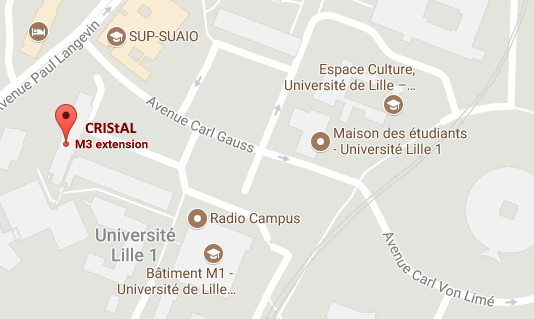
\includegraphics[scale=0.4 , frame]{img/cristalLocation.png} 
	\caption{CRIStAL laboratory Location}
\end{figure}

%reference annex organigram + add cristal to image

\section{Research activities}

CRIStAL's research activities concern topics related to the major scientific and societal issues of the moment such as: Big Data, software, computer imaging, human-machine interactions, robotics, control and supervision of large systems, intelligent embedded systems, bioinformatics\dots The laboratory is involved in the development of revolutionary platforms such as Pharo, a pure object oriented language and a powerful yet simple development environment used worldwide.

\section{2XS team}

The 2XS (eXtra Small, eXtra Safe) team is working on highly constrained embedded devices, precisely on designing software and hardware that are secure, safe and efficient. Research in this team is focused on defining new system architectures or new languages to allow fast development of reliable embedded software. The team addresses issues concerning memory footprint, energy consumption and security and takes profit from proficiencies in formal verification, hardware/software co-design and operating system architectures to tackle the aforementioned issues.\\

The team is lead by \textit{Prof.Gilles Grimaud} and has 15 members\footnotemark[1] as well as several trainees and most of its current work mainly revolves around the PIP project and its applications.

\begin{figure}[!ht]
	\centering 
	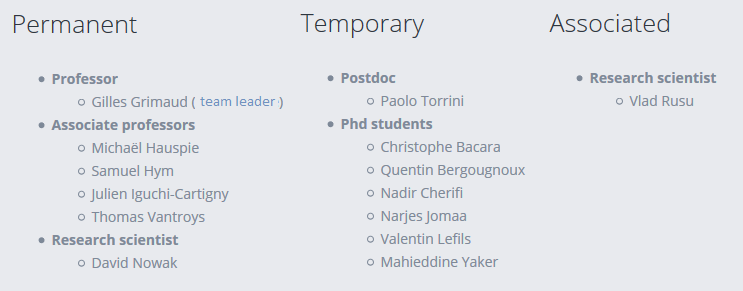
\includegraphics[width=\linewidth, frame]{img/2XS.png} 
	\caption[The 2XS team organizational chart]{The 2XS team organizational chart\cite{cristal}}
\end{figure}

% reference to PIP project section

\footnotetext[1]{as of \today}




 
\chapter{Background : PIP project}

\section{The PIP protokernel}

\subsection{A minimal OS kernel with provable isolation} \label{PIP}
An operating system is organized as a hierarchy  of layers \cite{ModernOS}, each one constructed  upon  the one  below. Each layer focuses on an essential role of the operating system such as memory management, multiprogramming and input/output. Generally speaking, while developing a kernel for an operating system based on the layered  approach, the designers have a choice where to draw the kernel-user boundary. Traditionally, all the layers went in the kernel, but that is not necessary. In fact, putting as little as possible in kernel mode is safer because kernel bugs can bring down the system instantly. In contrast, user processes/layers are set up to have less power so that a bug there may not be fatal.\\

Various studies on bug density, relatively to the developed module size, age as well as other factors, have been conducted (e.g.  \textit{Basilli}  and  \textit{Perricone} in 1984;  and \textit{Ostrand}  and  \textit{Weyuker} in 2002). A  ballpark  figure  for  serious industrial systems is ten  bugs per a thousand  lines  of code. Operating  systems  are  sufficiently  buggy  that  computer  manufacturers  put  reset  buttons  on  them, something  the  manufacturers of cars, TV sets and stereos do  not do,  despite  the  large  amount  of software in these devices. Furthermore, Operating systems generally present hardware resources to applications through high-level abstractions such as (virtual) file systems.\\

\noindent Therefore, we can distinguish several OS kernel families such as : 
\begin{itemize}
	\item \textbf{Monolithic kernels :}  All the OS layers are put in kernel space as in Windows and Linux;
	\item \textbf{Microkernels :} The basic idea  behind a microkernel design  is  to  achieve high reliability  by  splitting the operating  system  up into small, well-defined  modules, only  one  of  which, the  microkernel, runs  in  kernel  mode;
	\item \textbf{Exokernels :} The idea behind an exokernel is to force as few abstractions as possible on application developers, enabling them to make as many decisions as possible about hardware abstractions.
\end{itemize} 

As a \textbf{minimal OS Kernel with provable isolation}, PIP \cite{PIP} focuses more on security and safety without sacrificing efficiency and ensures memory isolation between different tasks running on the same device. PIP's algorithmic part is written in Gallina, the language of the Coq proof assistant, in a monadic style that allows direct translation into free standing C. We will refer to this implementation in \textit{Gallina} as the shallow embedding in contrast to the deep embedding introduced in section \ref{deep} p.\pageref{deep}. \\
  
Although the closest kernel design to PIP is the exokernel \cite{PIPSlides}, PIP does not belong to any of the kernel families featured in the state of art, but it is the first member of a new kernel family, \textbf{protokernels}, as compared to most microkernels and exokernels, the TCB in PIP is even more restricted :
\begin{itemize}
	\item Scheduling and IPC are done in user mode unlike a microkernel;
	\item Multiplexing is also done in user mode unlike an exokernel.
\end{itemize}

\noindent whereas the kernel mode is only for \textbf{multi-level MMU control and configuration} (virtual memory) and \textbf{context switching}. This not only ensures less bugs but also more feasibility of formal proof that will warrant the memory isolation property of the protokernel.

\begin{figure}[!ht]
	\centering 
	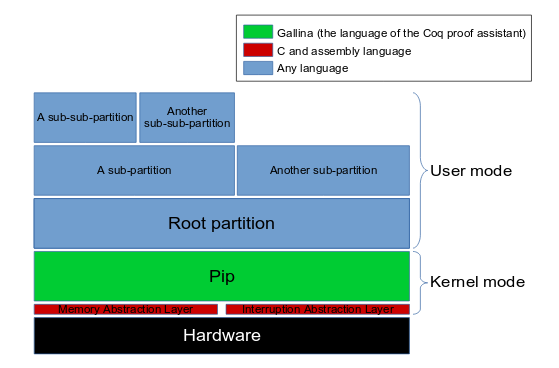
\includegraphics[width=0.9\linewidth ,frame]{img/OSLayersPIP.png} 
	\caption[Software layers of an OS built on top of PIP]{Software layers of an OS built on top of PIP \cite{PIPSlides}}
\end{figure}

\subsection{Horizontal isolation \& vertical sharing} \label{properties}

PIP can be used to partition the available memory which will be initially allocated to the root partition on top of PIP. Any partition can read and write in the memory of its descendants. However, partitions in different branches of the partition tree are disjoint. The former is referred to as \textbf{vertical sharing} and the latter as \textbf{horizontal isolation} \cite{PIPKernel}. Needless to say, all memory lent to PIP for storing kernel data,such as when creating partitions, is inaccessible for all partitions to prevent messing up PIP data structures which means that the kernel data is totally isolated.
   
\begin{figure}[!ht]
	\centering 
	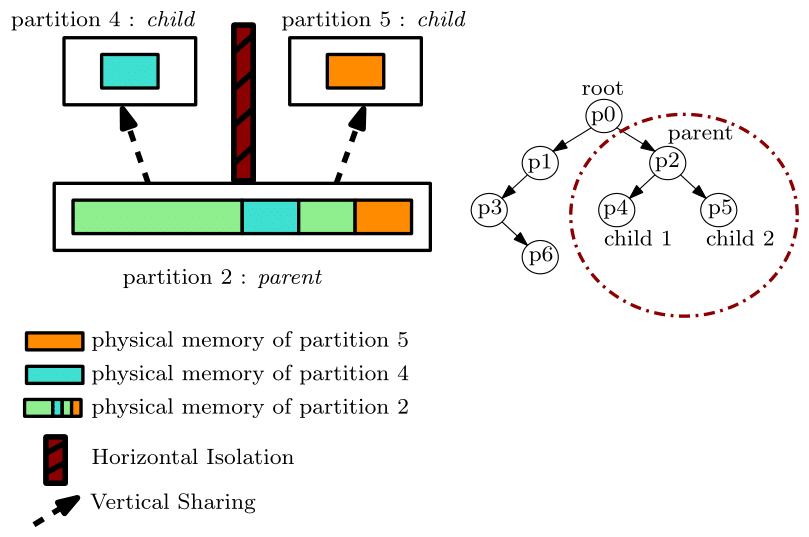
\includegraphics[width=0.8\linewidth,frame]{img/memoryIsolShare.png} 
	\caption[Horizontal isolation \& vertical sharing in PIP]{Horizontal isolation \& vertical sharing in PIP \cite{PIPKernel}}
\end{figure}

\noindent Let us consider a more realistic partition tree, as shown in figure \ref{FreeRTOS}, in which we consider \textit{Linux} and \textit{FreeRTOS} as sub-partitions of a root partition, multiplexer. Knowing that \textit{FreeRTOS} is a real-time OS that does not isolate its tasks, we have easily secured it with task isolation by porting it on PIP.

\begin{figure}[!ht] \label{FreeRTOS}
	\centering 
	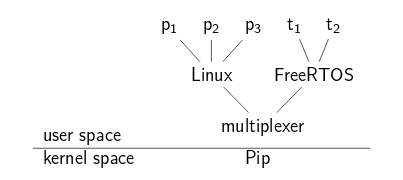
\includegraphics[scale=0.5,frame]{img/FreeRTOSEx.png} 
	\caption[FreeRTOS task isolation using PIP]{FreeRTOS task isolation using PIP \cite{PIPSlides}}
\end{figure}

\subsection{Proof-oriented design}

\subsubsection{PIP's design} 
PIP's isolation properties are meant to be formally proven independently from the platform it's running onto. Consequently, the algorithm and the architecture dependant part were separated \cite{PIPKernel}. Indeed, as shown in figure \ref{design}, PIP is split into two distinct layers  :
\begin{itemize}
	\item \textbf{HAL :} gives direct access to the architecture and hardware;
	\item \textbf{API :} implements the algorithmic part to configure the virtual memory and the hardware.
\end{itemize}

\noindent The API code is written and proven using the Coq proof assistant, and uses the interface provided by the HAL to perform any hardware related operation. the proofs are based on Hoare logic theory introduced in section \ref{Hoare} p.\pageref{Hoare}.

\begin{figure}[!ht]  
	\centering 
	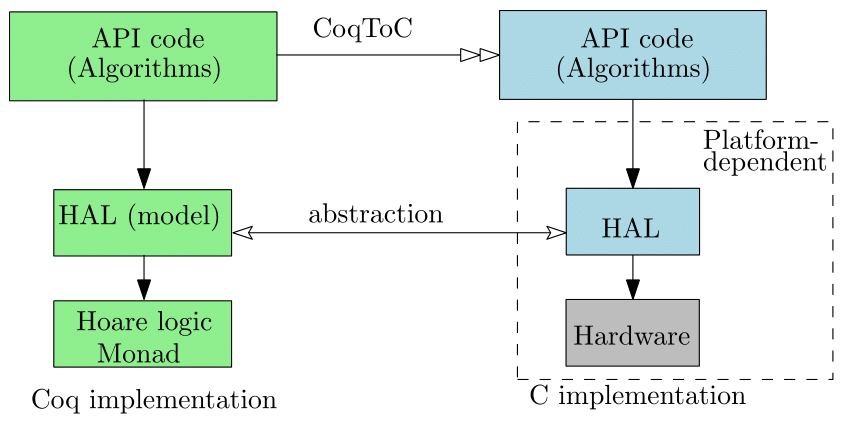
\includegraphics[width=0.8\linewidth, frame]{img/PIPDesign.png} 
	\caption[PIP design]{PIP design \cite{PIPKernel}}
	\label{design}
\end{figure}

\noindent PIP's HAL is split into three components, as shown in figure \ref{HAL}, each handling a specific part of the target platform's hardware :
\begin{itemize}
	\item \textbf{\gls{MAL} :} provides an interface for the configuration of the MMU chip (\cite{PIP}, MAL.v, MALInternal.v);
	\item \textbf{\gls{IAL} :} provides an interface to dispatch interrupts and configure hardware;
	\item \textbf{Bootstrap :} contains the low-level code required to boot the system.
\end{itemize}

\noindent PIP only provides system calls for management of the partitions and for context switching, thus reducing the TCB to its bare minimum as explained in section \ref{PIP} p.\pageref{PIP}. This user exposed API (\cite{PIP}, Services.v) can be called by any partition using a platform dependant call :
\begin{itemize}
	\item \textbf{createPartition :} creates a new child (sub-partition) into the current partition;
	\item \textbf{deletePartition :} removes a child partition and puts all its used pages back in the current partition;
	\item \textbf{prepare :} adds required configuration tables into a child partition to map a new virtual address;
	\item \textbf{collect :} removes the empty configuration tables which are not used anymore and gives it back to the current partition; 
	\item \textbf{countToMap :} returns the amount of configuration tables needed to perform a mapping for a given virtual address;
	\item \textbf{addVaddr :} maps a virtual address into the given child;
	\item \textbf{removeVAddr :} removes a given mapping from a given child.
\end{itemize} 
This API is sufficient as far as memory requirements are concerned but it lacks a way to handle interrupts. Hardware interrupts are implicitly handled by PIP and automatically dispatched to the root partition, while software interrupts, such as system calls, are notified to the parent partition of the caller \cite{PIPKernel} and can be managed by these two additional services of PIP :
\begin{itemize}
	\item \textbf{dispatch :} notifies an interrupt to a given partition, interrupting its current control flow and backing it up for a further resume call;
	\item \textbf{resume :} restores a previously interrupted context.
\end{itemize}
\vspace{-0.8em} 
\begin{figure}[!ht]  
	\centering 	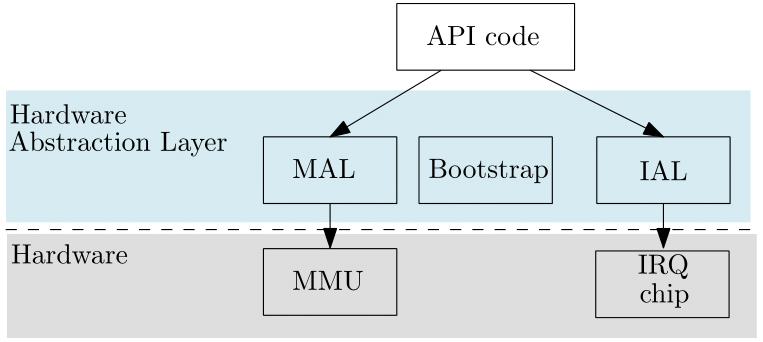
\includegraphics[width=0.58\linewidth,frame]{img/HAL.png} 
	\caption[HAL and API relationship]{HAL and API relationship \cite{PIPKernel}}
	\label{HAL}
\end{figure}

\subsubsection{Formal proofs using Coq} 
\begin{wrapfigure}[6]{r}{0.2\textwidth}
\vspace{-14pt}
\centering

\includegraphics[frame]{img/CoqLogo.png}
\end{wrapfigure}
Coq \cite{CoqWeb} is the result of about 30 years of research. It started in 1984 as an implementation of the Calculus of Constructions, an expressive formal language, at INRIA by \textit{Thierry Coquand} and \textit{G\'erard Huet} and was extended, later in 1991, by \textit{Christine Paulin} to the Calculus of Inductive Constructions \cite{Calculus}. \\

Coq is a \textbf{formal proof management system}. It provides a formal language to write mathematical definitions, executable algorithms and theorems together with an environment for semi-interactive development of machine-checked proofs. Typical applications include the certification of properties of programming languages (e.g. the \textit{CompCert} compiler certification project, or the \textit{Bedrock} verified low-level programming library), the formalization of mathematics and teaching. It implements a program specification and mathematical higher-level language called \textit{Gallina} that is based on the Calculus of Inductive Constructions combining both a higher-order logic and a richly-typed functional programming language.\\

As a \textbf{proof development system}, Coq provides interactive proof methods, decision and semi-decision algorithms as well as a tactic language letting the user define his own proof methods. Furthermore, as a \textbf{platform for the formalization of mathematics or the development of programs}, Coq provides support for high-level notations, implicit contents and various other useful kinds of macros.\\

For this project, the latest version of Coq, 8.6 released in December 2016, was used. It features among other things a faster universe checker, asynchronous error processing, proof search improvements, generalized introduction patterns, a new warning system and subterm selection algorithm. \\

The Coq proof assistant provides us with powerful tactics to perform proofs \cite{Coq}. Here is a non exhaustive list of these tactics :
\begin{itemize}
\item \textbf{simpl :} simplifies the current goal;
	\item \textbf{assumption :} solves the current goal if it is computationally equal to a hypothesis;
	\item \textbf{reflexivity :} solves the current goal if it is a valid equality;
	\item \textbf{unfold t :} unfolds the definition of t in the current goal;
	\item \textbf{clear H :} removes hypothesis H from the context;
	\item \textbf{auto :} tries to solve the current goal automatically by using a collection of tactics;
	\item \textbf{rewrite H :} uses an equality hypothesis H to replace a term in the current goal;	
	\item \textbf{induction t:} applies the induction principle for the type of t, generates subgoals as many as there are constructors, and adds the inductive hypotheses in the contexts;
	\item \textbf{inversion H :} resembles the induction tactic, but pays attention to the particular form of the type of H, and will only consider the cases that could have been used, so it discards some impossible cases quickly and efficiently;
	\item \textbf{omega :} carries out an automatic decision procedure for \textit{Presburger} arithmetic;
	\item \textbf{apply H :} mainly tries to unify the current goal with the conclusion of the type of H. If it succeeds, then the tactic returns as many subgoals as non-dependent premises of the type of H;
	\item \textbf{f\_equal :} applies to a goal of the form $f$ a{\tiny 1} \dots a{\tiny n} = $g$ b{\tiny 1} \dots b{\tiny n} and leads to subgoals $f = g$ and a{\tiny 1} = b{\tiny 1} and so on up to a{\tiny n} = b{\tiny n}. Amongst these subgoals, the simple ones are automatically solved;
	\item \textbf{contradiction :} tries to find a contradiction amongst the hypotheses.	
\end{itemize}
Coq also provides several tactics to deal with higher-order logic, particularly targeting binary connectives and quantifiers such as \textbf{split} for conjunction, \textbf{left} and \textbf{right} for disjunction, \textbf{intros} for implication and universal quantifiers and \textbf{exists} for existential quantifiers when they are in the goal. In addition, We have \textbf{destruct} for conjunction and disjunction, \textbf{apply} for implication, \textbf{elim} for existential quantifiers and \textbf{specialize} for universal quantifiers when they are in the hypothesis. Furthermore, many tactics can be preceded with the letter \textit{e} like \textbf{eauto}, \textbf{eassumption} and \textbf{eapply} to deal with existential variables. Some tactics can also be applied on hypotheses if we use the reserved clause \textit{in} with the name of the hypothesis such as unfold, apply and simpl. 
%ref Curry , In throry, \textbf{proving is the same as programming}. 

\subsection{In-depth understanding of PIP's data structures} \label{structures}

\subsubsection{The memory}

PIP uses several data structures per partition \cite{PIPKernel}, which will represent the global state of the partition's memory state. This is necessary as it has to keep track of pages allocated to partitions in order to allow or deny derivation and partition creation while preserving the required properties. \\

Figure \ref{partitionEx} shows a partition tree example consisting of a partition, Parent, that has a single child, Child1. A partition is identified by a partition descriptor which is a page number essential to access the whole data structure of a partition. In our case, the partition descriptors of Parent and Child1 are respectively 1 and 12. The pages lent to PIP to manage a partition are organized in a tree with three branches : the MMU tables, the first shadow and the second shadow. The aim of this organization is to keep additional information about each page lent to a partition. Moreover these structures have multiple goals :
\begin{itemize}
	\item \textbf{Access control :} the first shadow is used to avoid deriving the same page multiple times;
	\item \textbf{Performance :} the second shadow and the configuration list are used to quickly find the virtual address of a page without having to parse the whole virtual space when the parent partition reclaims it.
\end{itemize} 
As such, adding an indirection table in the MMU configuration requires two additional pages for the shadows. Therefore, this model is estimated to require roughly three times the amount of memory a simple virtual environment would need, nevertheless it provides a  secure and an efficient API. \\

To prove the isolation properties on this memory structure, it is essential to ensure its consistency relative to the partition tree, the well-typedness as well as some other consistency properties that will be detailed in section \ref{Hoare} p.\pageref{Hoare}.

\vfill 

\begin{figure}[!ht]  
	\centering 
	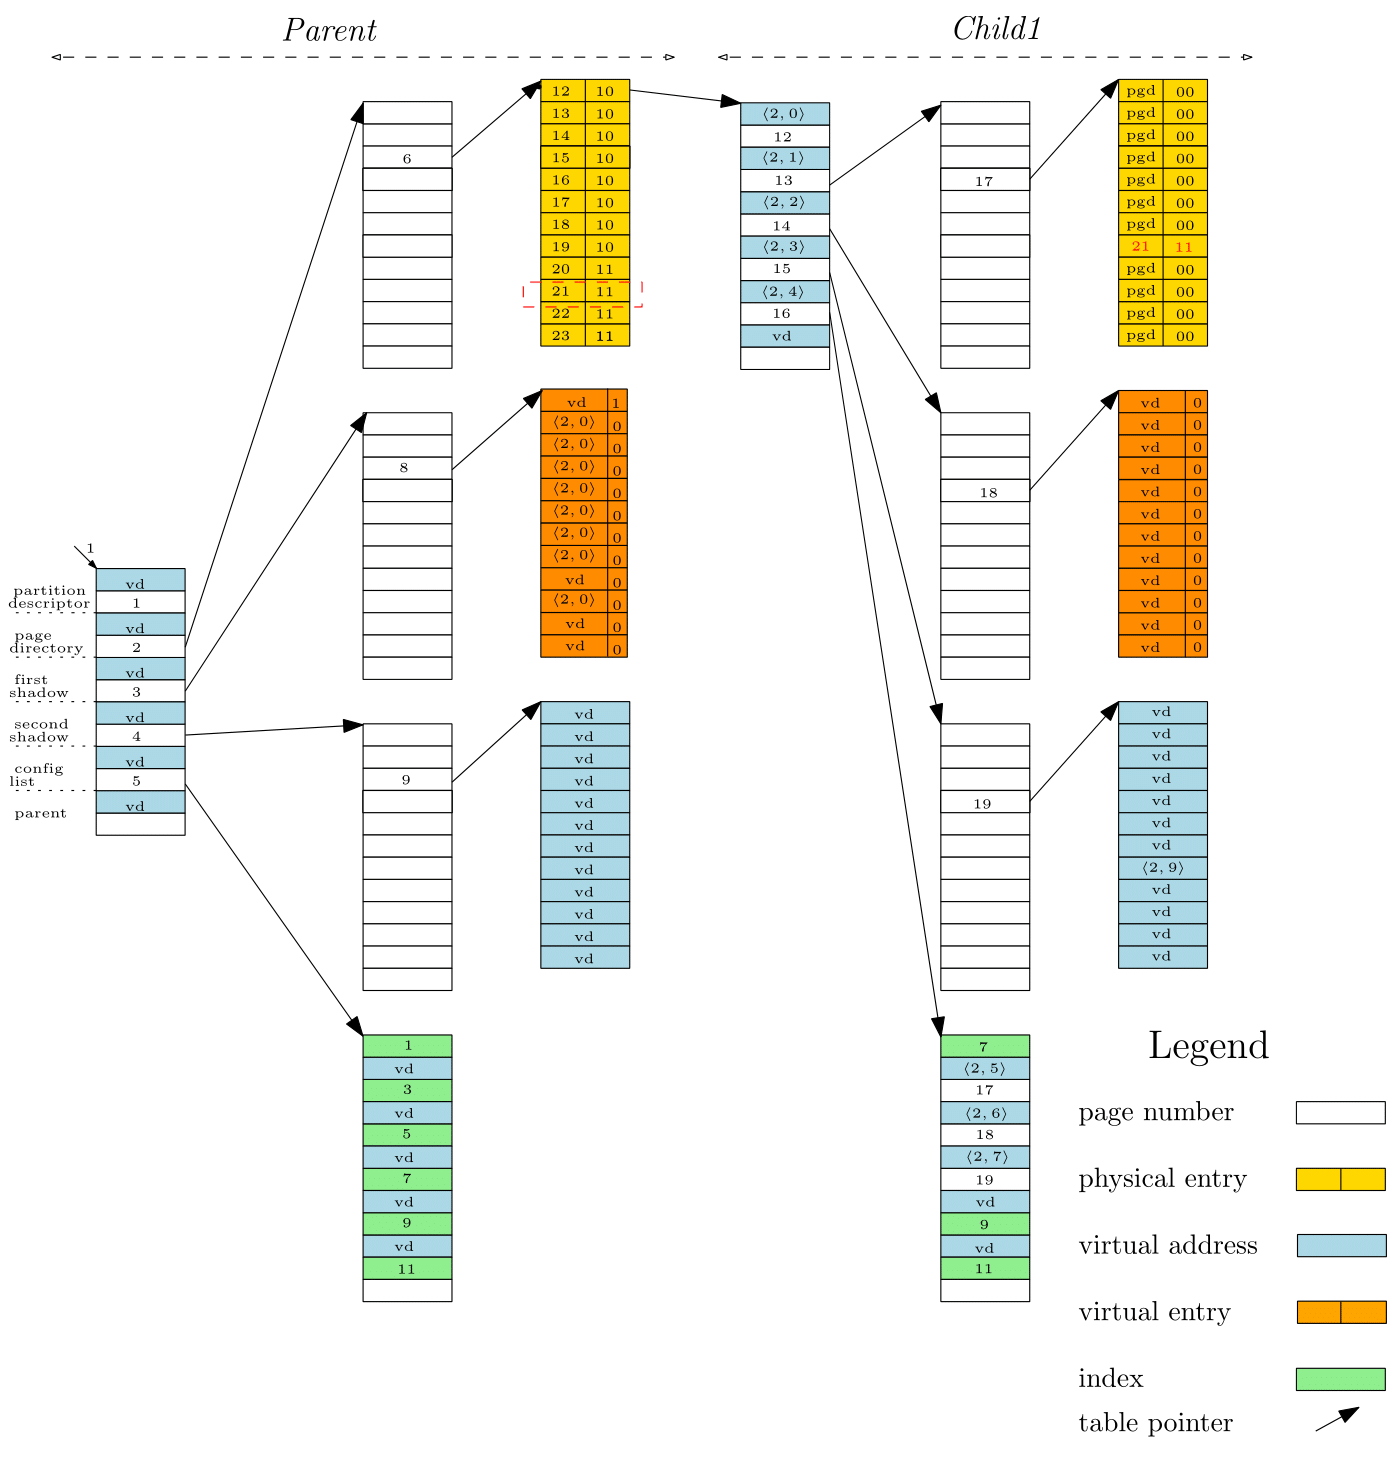
\includegraphics[width=1\linewidth, height=0.6\textheight, frame]{img/memoryEx.png} 
	\caption[An example of a partition tree]{An example of a partition tree \cite{PIPKernel}}
	\label{partitionEx}
\end{figure}

\subsubsection{The memory state} \label{PIPstateSection}
 
\noindent The PIP memory state \cite{PIPdraft} (\cite{PIP}, ADT.v, Hardware.v) is defined as follows :
\begin{lstlisting}[linewidth=1.02\linewidth,caption = {PIP state definition},label={PIPstate}] 
Record state : Type := 
{ currentPartition: page ; memory: list (paddr * value) }.
\end{lstlisting}
The list in the state corresponds to the physical memory and maps physical addresses to values. A physical address is defined by a physical page number and a position into this page :
\begin{lstlisting}[caption = {paddr type definition},xleftmargin=.15\textwidth,xrightmargin=.15\textwidth] 
Definition paddr : Type := page * index.
\end{lstlisting}
where pages and indexes are positive integers bounded respectively by the overall number of pages and the table size :
\begin{lstlisting}[caption = {page \& index type definitions},xleftmargin=.05\textwidth,xrightmargin=.05\textwidth]
Record page := { p :> nat ; Hp : p < nbPage }. 
Record index := { i :> nat ;  Hi : i < tableSize }.
\end{lstlisting}
Different types of values could be stored in the physical memory by Pip. So, the type \textit{value} is an inductive type defined as follows :
\begin{lstlisting}[caption = {value type definition}, mathescape=true,xleftmargin=.23\textwidth,
xrightmargin=.23\textwidth]
Inductive value : Type :=
	| PE: Pentry $\rightarrow$ value
	| VE: Ventry $\rightarrow$ value
	| PP: page   $\rightarrow$ value
	| VA: vaddr  $\rightarrow$ value
	| I:  index  $\rightarrow$ value.
\end{lstlisting}
The type \textit{Pentry}, which represents a physical entry, consists of a physical page number along with several flags :
\begin{lstlisting}[caption = {Pentry type definition},xleftmargin=.27\textwidth,
xrightmargin=.27\textwidth]
Record Pentry : Type := {
  	read:    bool ;
   	write:   bool ;
   	exec:    bool ;
   	present: bool ;
   	user:    bool ;
   	pa:      page }.
\end{lstlisting}
Finally, the \textit{Ventry} type consists of a virtual address with a boolean flag :
\begin{lstlisting}[caption = {Ventry type definition},xleftmargin=.06\textwidth,xrightmargin=.06\textwidth]
Record Ventry : Type := { pd: bool ; va: vaddr }.
\end{lstlisting}
with virtual addresses modelled as a list of indexes of length the number of levels of the MMU plus one :
\begin{lstlisting}[caption = {vaddr type definition},xleftmargin=.02\textwidth,xrightmargin=.02\textwidth]
Record vaddr : Type := 
{ va :> list index ; Hva : length va = nbLevel + 1  }.
\end{lstlisting}

\subsubsection{The PIP monad}

The previous memory state definition is used to define a monad, called \textit{LLI}, that performs the computation of PIP programs. When we execute a PIP program function starting from a certain memory state, we are not only interested in its resulting value but also in the resulting state. This is essential for stateful operations which modify the memory state. It is also important to deal with undefined behaviour. The \textit{LLI} ensures all of these specifications and is defined as follows (\cite{PIP},Hardware.v) : 
\begin{lstlisting}[caption = {PIP LLI monad},xleftmargin=-.06\textwidth,xrightmargin=-.06\textwidth,label=monad,mathescape=true]
Inductive result (A : Type) : Type :=
| val : A $\rightarrow$ result A
| undef : nat $\rightarrow$ state $\rightarrow$ result A.

Definition LLI (A :Type) : Type := state $\rightarrow$ result (A * state).
\end{lstlisting}

\noindent Using the LLI monad, some instructions were explicitly defined as follows (\cite{PIP},Hardware.v) : 
\begin{lstlisting}[caption = {Explicitly defined instructions in the shallow embedding},xleftmargin=-.02\textwidth,xrightmargin=-.02\textwidth,label=shallowIns,mathescape=true]
(*Return instruction*)
Definition ret {A : Type} (a : A) : LLI A :=
  fun s $\Rightarrow$ val (a , s) .

(*Assignment instruction*)
Definition bind {A B : Type} (m : LLI A) 
	        (f : A $\rightarrow$ LLI B) : LLI B :=  
  fun s $\Rightarrow$ match m s with
    | val (a, s') $\Rightarrow$ f a s'
    | undef a s' $\Rightarrow$ undef a s'
    end.

(*Skip instruction*)
Definition put (s : state) : LLI unit :=
  fun _ $\Rightarrow$ val (tt, s).

(*For undefined behaviour*)
Definition undefined {A : Type} (code : nat) : LLI A :=
  fun s $\Rightarrow$ undef code s.
\end{lstlisting}
\section{Hoare logic}

\subsection{Introduction to Hoare logic theory} \label{HoareIntro}
\textit{How can we argue that a program is correct ?}
Nowadays, Building reliable software is becoming more and more difficult considering the growing scale, specifications and complexity of modern systems. Therefore, tests alone can no longer ascertain the reliability of programs especially if we're talking about critical systems. Logicians, computer scientists and software engineers have responded to these challenges by developing different kinds of techniques some of which are based on formal reasoning about properties of software and tools for helping validate these properties. One of these reasoning techniques that was used to prove PIP's properties is \textit{Floyd–Hoare logic}, often shortened to just \textbf{Hoare Logic}. It was proposed in 1969 by the British computer scientist and logician Tony Hoare \cite{Hoare} and it continues to be the subject of intensive research right up to the present day. It is not only a natural way of \textbf{writing down specifications of programs} but also a technique for \textbf{proving that programs are correct} with respect to such specifications. A Coq implementation of Hoare logic on a simple imperative programming language called Imp is explained in \textit{Software Foundations} \cite{SoftwareFoundation}. \\  % other technique : Model checking 

Let S be a program that we want to execute starting from a certain state s, P a predicate on the state describing the condition S relies on for correct execution and Q a predicate on the resulting state after the execution of S describing the condition S establishes after correctly running. Knowing that P is verified on s, if we prove that Q is verified after the execution of s, we can ascertain that S is partially correct. And by partial correctness of S we mean that S is correct if it terminates. Using standard Hoare logic, only partial correctness can be proven, while termination needs to be proven separately. This triple S, P and Q, written as \textbf{ \{P\} S \{Q\} }, is referred to as a \textbf{Hoare triple}. The assertions P and Q are respectively referred to as the \textbf{precondition} and the \textbf{postcondition}. \\

\noindent For example let's consider simple Hoare triples about an assignment command :
\begin{itemize}
	\item \boldmath$\{X=2\} X:=X+1 \{X=3\}$ : is a valid Hoare triple, that can be easily formally proved in Coq, since the postcondition is verified after the execution of the assign command relatively to the precondition;
	\item \boldmath$\{X=2\} X:=X*2 \{X=3\}$ : is not a valid Hoare triple since the postcondition would not be verified after the execution of the command.
\end{itemize} 
\pagebreak
\noindent Now, let's introduce some facts and rules about Hoare triples :
\begin{enumerate}
\item If an assertion P implies another precondition P' of a valid Hoare triple \{P'\} S \{Q\} then \{P\} S \{Q\} is also a valid Hoare triple. This is referred to as \textbf{weakening the precondition of a Hoare triple} and can be formally defined as follows :
\vspace{-10pt}
\begin{prooftree}
\AxiomC{P $\rightarrow$ P'}
\AxiomC{\{P'\} S \{Q\}}
\RightLabel{\small{Hoare\_weaken}}
\BinaryInfC{\{P\} S \{Q\}}
\end{prooftree}
\item If we can weaken a Hoare triple, we expect it to have a \textbf{weakest precondition}. This notion was introduced by Dijkstra in 1976 \cite{DIJ} and is very important since it enables us to prove total correctness and in particular program termination. Indeed, if a program doesn't terminate, its weakest precondition would be \textit{True} and it would verify any postcondition.
\item If we consider a language containing a \textbf{SKIP instruction} which practically does nothing, we can affirm that this command preserves any property which means :
\vspace{-15pt}
\begin{prooftree}
\AxiomC{}
\RightLabel{\small{Hoare\_skip}}
\UnaryInfC{\{P\} SKIP \{P\}}
\end{prooftree}
\item If we consider a language that allows \textbf{assignments}, in the form of \linebreak \emph{X := a}, then we can conclude that an arbitrary property Q holds after such assignment if we assume Q[X$\rightarrow$a] which means Q with all occurrences of X replaced by a :
\vspace{-10pt}
\begin{prooftree}
\AxiomC{}
\RightLabel{\small{Hoare\_assign}}
\UnaryInfC{\{Q[X$\rightarrow$a]\} X:= a \{Q\}}
\end{prooftree}
\item Generally speaking, every Program is built using \textbf{sequencing} of commands that we will write as C1\textbf{;}C2. Our aim is to prove a Hoare triple on this sequence with P and Q respectively as the precondition and the postcondition. This requires proving that C1 takes any state where P holds to a state where an intermediate assertion I holds and C2 takes any state where I holds to one where Q holds which could be formally stated as :
\vspace{-10pt}
\begin{prooftree}
\AxiomC{\{P\} C1 \{I\}}
\AxiomC{\{I\} C2 \{Q\}}
\RightLabel{\small{Hoare\_seq}}
\BinaryInfC{\{P\} C1\textbf{;}C2 \{Q\}}
\end{prooftree}
\item Finally, let's not forget \textbf{conditional structures} that we can write in the form of \emph{IF B THEN C1 ELSE C2}. To verify a Hoare triple about this instruction with P and Q respectively as the precondition and postcondition, we need to consider both cases where B is evaluated to \textit{true} and \textit{false} and prove that Q holds on the resulting state in each one. We can also disregard a case if there is some sort of contradiction relatively to the property P. This rule can be written as follows :
\vspace{-10pt}
\begin{prooftree}
\AxiomC{\{P $\bigwedge$ B\} C1 \{Q\}}
\AxiomC{\{P $\bigwedge \neg$ B\} C2 \{Q\}}
\RightLabel{\small{Hoare\_if}}
\BinaryInfC{\{P\} IF B THEN C1 ELSE C2 \{Q\}}
\end{prooftree}
\end{enumerate}
The rules defined above are in their simplest form and we need to adapt them to the language or semantics we are working on. Also, This list is not exhaustive. For example, we did not define a rule for \textit{While} loops because the Coq model of PIP doesn't actually use them and uses recursion instead. Likewise, We are sure that all PIP's functions terminate since recursive functions are bounded by a maximum number of iterations.  

\subsection{Hoare logic in the shallow embedding} \label{Hoare}
The Hoare logic devised for the shallow embedding is slightly different from what we saw in the previous section \cite{MMUIsolation}. A program in the shallow embedding is defined in a monadic style that returns a pair of values, the first being the resulting state and the second the value returned by the program which generally corresponds to a function. Thus, as shown in script \ref{shallow_Hoare} (\cite{PIP}, Hardware.v), \textbf{the postcondition is a predicate on the resulting state and the returned value} so that we can verify it and propagate it in the case of long proofs. The notation chosen for the Hoare triple stays the same as the one mentioned in the previous section except for the brackets that are doubled since single brackets are already used in Coq.
\begin{lstlisting}[caption = {Hoare triple in the shallow embedding},label = {shallow_Hoare}, mathescape=true,xleftmargin=.02\textwidth,
xrightmargin=.02\textwidth]
Definition hoareTriple {A : Type} (P : state $\rightarrow$ Prop) 
(m : LLI A) (Q : A $\rightarrow$ state $\rightarrow$ Prop) : Prop :=
  $\forall$ s, P s $\rightarrow$ match (m s) with
    | val (a, s') => Q a s'
    | undef _ _=> False
    end.

Notation "{{ P }} m {{ Q }}" := (hoareTriple P m Q)
  (at level 90, format "'[' '[' {{  P  }}  ']' '/  '
  '[' m ']' '['  {{  Q  }} ']' ']'") : state_scope.
\end{lstlisting}
The weakening lemma, extensively used in PIP's proofs, was also defined and proven in the following script (\cite{PIP}, WeakestPreconditions.v) :
\begin{lstlisting}[caption = {Weakening Hoare triples in the shallow embedding},label = {shallow_weaken}, mathescape=true,xleftmargin=.06\textwidth,
xrightmargin=.06\textwidth]
Lemma weaken (A : Type) (m : LLI A) 
(P Q : state $\rightarrow$ Prop) (R : A $\rightarrow$ state $\rightarrow$ Prop) :
  {{ Q }} m {{ R }} $\rightarrow$ 
  ($\forall$ s, P s $\rightarrow$ Q s) $\rightarrow$
  {{ P }} m {{ R }}.
Proof.
intros H1 H2 s H3.
case_eq (m s); [intros [a s'] H4 | intros a H4 ];
apply H2 in H3; apply H1 in H3; 
try rewrite H4 in H3; trivial.
intros. rewrite H in H3. assumption. 
Qed.
\end{lstlisting}
Some instructions were considered as primitive like conditional structures while some others were explicitly defined like assignments, in the form of \textit{\textbf{perform x := m in e}} where the value of the program m gets assigned to x in the evaluation of the program e, defined in script \ref{shallowIns} p.\pageref{shallowIns}. Furthermore, a Hoare triple rule was devised for assignments as follows (\cite{PIP}, WeakestPreconditions.v) :
\begin{lstlisting}[caption = {Hoare triples assignment rule in the shallow embedding},label = {shallow_assign},mathescape=true]
Lemma bind (A B : Type) (m : LLI A) (f : A $\rightarrow$ LLI B) 
(P : state $\rightarrow$ Prop) ( Q : A $\rightarrow$ state $\rightarrow$ Prop) 
(R : B $\rightarrow$ state $\rightarrow$ Prop) :
  ($\forall$ a, {{ Q a }} f a {{ R }}) $\rightarrow$ 
  {{ P }} m {{ Q }} $\rightarrow$ 
  {{ P }} perform x := m in f x {{ R }}.
Proof. 
intros H1 H2 s H3; unfold bind;
case_eq (m s); [intros [a s'] H4 | intros k s' H4];
apply H2 in H3; rewrite H4 in H3; trivial.
case_eq (f a s'); [intros [b s''] H5 | intros k s'' H5];
apply H1 in H3; rewrite H5 in H3; trivial.
Qed. 
\end{lstlisting}

Finally, to reason with Hoare logic we need to formally  specify the properties we want to prove \cite{PIPKernel}, the most important being partition memory isolation,
kernel data isolation, vertical sharing and consistency mentioned in \ref{properties} p.\pageref{properties}. To that end, the following necessary functions on PIP's data structures were defined (\cite{PIP}, StateLib.v) : 
\begin{itemize}
	\item \textbf{getChildren :} returns the list of all children of a given parent partition in the partition tree of a given state;
	\item \textbf{getAncestors :} returns the list of all ancestors of a given partition in the partition tree of a given state;
	\item \textbf{getMappedPages :} returns the list of mapped pages of a given partition;
	\item \textbf{getAccessibleMappedPages :} returns the list of all mapped pages, of a given partition, marked as accessible;
	\item \textbf{getUsedPages :} returns the list of all the pages that are used by a given partition including the pages lent to PIP;
		\item \textbf{getConfigPages :} returns the list of configuration pages lent to PIP to manage a given partition;
	\item \textbf{getPartitions :} returns the list of all existing partitions of a given state which is naturally obtained by a search on the partition tree.
\end{itemize} 
The first property defines horizontal isolation between children i.e., for any state s of the system, all memory pages owned by two different children of a given parent partition in the partition tree must be distinct. This property is formally defined in the Coq proof assistant as follows (\cite{PIP}, Isolation.v) :
\begin{lstlisting}[caption = {Horizontal isolation}, mathescape=true,xleftmargin=.02\textwidth,
xrightmargin=.02\textwidth]
Definition horizontalIsolation s :=
$\forall$ parent child1 child2,
parent $\in$ getPartitions s $\rightarrow$
child1 $\in$ getChildren parent s $\rightarrow$
child2 $\in$ getChildren parent s $\rightarrow$
child1 $\neq$ child2 $\rightarrow$
(getUsedPages child1 s) $\cap$ (getUsedPages child2 s) = $\emptyset$.
\end{lstlisting}
The second property defines vertical sharing between a parent partition and its children i.e. it ensures that all pages mapped by a child are mapped in its parent. This property is formally defined as follows (\cite{PIP}, Isolation.v) :
\begin{lstlisting}[caption = {Vertical sharing}, mathescape=true,xleftmargin=.08\textwidth,
xrightmargin=.08\textwidth]
Definition verticalSharing s :=
$\forall$ parent child,
parent $\in$ getPartitions s $\rightarrow$
child $\in$ getChildren parent s $\rightarrow$
getUsedPages child s $\subseteq$ getMappedPages parent s.
\end{lstlisting}
The third property defines kernel data isolation meaning it ensures that for any state of the system and any given two possibly-equal partitions, the code running in the second partition cannot access the pages containing configuration tables lent to PIP to manage the first partition. This property is formally defined as follows (\cite{PIP}, Isolation.v) :
\begin{lstlisting}[caption = {Kernel data isolation}, mathescape=true,xleftmargin=.12\textwidth,
xrightmargin=.12\textwidth]
Definition kernelDataIsolation s :=
$\forall$ partition1 partition2,
partition1 $\in$ getPartitions s $\rightarrow$
partition2 $\in$ getPartitions s $\rightarrow$
(getAccessibleMappedPages partition1 s) $\cap$
(getConfigPages partition2 s) = $\emptyset$.
\end{lstlisting}
The last property of consistency is mandatory to prove the previously detailed properties . Consistency encompasses different sub-properties that were divided into four categories. As the definition of this property is quite cumbersome, we will only disclose these categories and illustrate each one with an example (\cite{PIP}, Consistency.v):
\begin{itemize}
	\item \textbf{Partition tree structure :} the properties in this category ensure that the partition tree of a given state is consistent relatively to its awaited structure preset in section \ref{structures} p.\pageref{structures}. For example, one of the properties defined in this category and called \textit{noCycleInPartitionTree} ensures that there is no cycle in the partition tree of a given system i.e. each partition is different from all its ancestors in the partition tree. This property is formally defined as follows :
\begin{lstlisting}[caption = {Example of partition-tree-consistency property}, mathescape=true,xleftmargin=.08\textwidth,
xrightmargin=.14\textwidth]
Definition noCycleInPartitionTree s :=
$\forall$ ancestor partition,
partition $\in$ getPartitions s $\rightarrow$
ancestor $\in$ getAncestors partition s $\rightarrow$
ancestor $\neq$ partition.
\end{lstlisting}
	\item \textbf{Flag semantics :} This category focuses on the signification of flags used in the data structures. For instance, a property called \textit{isPresentNotDefaultIff} states that the associated page number of a physical entry whose \textit{present} flag is set to \textit{false}, corresponds to the predefined default page value. This property is formally defined as shown in script \ref{flags} where \textit{readPhyEntry} and \textit{readPresent} are predefined functions that respectively read, for a given table, index and memory state, the present flag of a physical entry and its value  :
\begin{lstlisting}[caption = {Example of a flags-semantics-consistency property}, mathescape=true , label={flags}]
Definition isPresentNotDefaultIff s :=
$\forall$ table idx,
readPresent table idx (s.memory) = Some false $\leftrightarrow$
readPhyEntry table idx (s.memory) = Some defaultPage.
\end{lstlisting}	 
	\item \textbf{Pages properties :} This category concerns several properties about the partitions' mapped pages, the pages lent to the kernel as well as the relations between them. For example, the \textit{noDupMappedPagesList} requires that the mapped pages of partitions be distinct from each other, using the function \textit{NoDup} which verifies whether a list contains duplicates or not. This property is formally defined as follows  :
\begin{lstlisting}[caption = {Example of a pages-consistency property}, mathescape=true,xleftmargin=.07\textwidth,
xrightmargin=.07\textwidth]
Definition noDupMappedPagesList s :=
$\forall$ partition, partition $\in$ getPartitions s $\rightarrow$
NoDup (getMappedPages partition s).
\end{lstlisting}	
	\item \textbf{Well-typedness :} This last category concerns kernel data types and ensures that PIP doesn't contain any type confusion. For instance, when PIP writes a virtual address in the memory, it should be read later as a virtual address which is ensured by a property called \textit{dataStructurePdSh1Sh2asRoot}. Otherwise, it is considered as an undefined behaviour in the model.
\end{itemize}
The most difficult system call invariant, called \textit{createPartition}, was successfully proven (\cite{PIP}, CreatePartition.v). It required about 60000 lines of code to prove. It is defined as follows :
\begin{lstlisting}[caption = {createPartition Hoare triple}, mathescape=true]
Lemma createPartition (descChild pdChild
           shadow1 shadow2 list : vaddr) :
{{fun s $\Rightarrow$ partitionsIsolation s  $\bigwedge$ kernelDataIsolation s 
	   $\bigwedge$ verticalSharing s $\bigwedge$ consistency s }} 
createPartition descChild pdChild shadow1 shadow2 list  
{{fun _ s  $\Rightarrow$ partitionsIsolation s $\bigwedge$ kernelDataIsolation 
              s $\bigwedge$ verticalSharing s $\bigwedge$ consistency s }}.
\end{lstlisting}	

\pagebreak

\section{The deep embedding} \label{deep}

\subsection{DEC}
DEC \cite{DEC} (Deep Embedding of a
terminating C-style language with effects) is a \gls{DSL} embedded in \textit{Gallina} and developed as an intermediate language for the translation of PIP to C. DEC Relies on Coq modules to define parametrisable state and identifiers types which are both specified in a module type (\textit{IdModType} shown in annex \ref{ModType} p.\pageref{ModType}). The dynamic semantics of DEC is specified in the small-step style of \gls{SOS}, introduced by \textit{Plotkin} \cite{SOS}, which formally describe how the individual steps of a computation take place enabling us to perform software verification by reasoning on formulas' structure. In small-step semantics, program behaviour is specified in terms of atomic steps and this makes it easier to specify constructs in dependently of one another \cite{TAOSD}. \\

\noindent The DEC language has the following properties (\cite{DEC}, README.txt) : 
\begin{enumerate}
	\item \textbf{Type soundness :} no well-typed program gets stuck on a
non-value, and when a well-typed program terminates it gives a value
of the right type;
	\item \textbf{Termination :} every execution of a well-typed program
ends with a value;
	\item \textbf{Subject reduction :} the execution of a well-typed
program preserves its type at each step;
	\item \textbf{Determinism :} given an initial state, each well-typed
program can only evaluate to one value and one new state;
	\item \textbf{Type uniqueness :} each program has at most one
type.	
\end{enumerate}
DEC supports Hoare logic reasoning, providing proven Hoare logic rules that will be detailed in section \ref{HoareDeepSec} p.\pageref{HoareDeepSec} (\cite{DEC}, THoare.v).

\iffalse
A deep embedding is mainly an \textbf{abstract representation of a language by modelling its expressions as data}. Strictly speaking, The main difference between a shallow and deep embedding is that the former is \textbf{ extensible with regards to adding language constructs} while the latter is \textbf{extensible with regards to adding interpretations of its abstract data types}. A typical approach in PIP's case would have been reasoning on a predefined deep embedding as structural abstraction enables us to perform cost-effective software verification by inversion on formulas' structure. However, defining such an abstract language, at the beginning, is quite tedious and rather intricate since we need to worry about the wingspan of such language and expression soundness among others. Therefore, the tasks of proof engineering and developing the deep embedding were separated. At first, a formal reasoning system based on Hoare logic was built on the shallow embedding as shown in section \ref{Hoare} p.\pageref{Hoare}. Then, an abstract representation of the shallow model was written in \textit{Gallina} which corresponds to the deep embedding. Needless to say, at some point later on, we need to worry about the preservation of proven properties between both embeddings either by proving that there is a bijection between them or by rewriting all the proofs in the deep embedding. By and large, we need to \textbf{ascertain the feasibility of such proofs in the deep embedding} as well as \textbf{compare examples of conducted proofs in both embeddings}.
\fi

\subsection{Deep embedding constructs}
\noindent Before we move on to the main constructs of the deep embedding, we need to introduce some essential background types and structures (\cite{DEC}, StaticSemA.v) :
\begin{itemize}
	\item \textbf{Id type :} represents the identifiers' type in the deep embedding. Typically, identifiers of variables are strings but we can use any other type;
	\item \textbf{Value type :} represents the actual values the programs will be manipulating. They can be built using the constructor \textit{cst} followed by a shallow type and a value that should be of that type. The value type and its constructor are defined as follows :
\begin{lstlisting}[caption = {Values in the deep embedding},xleftmargin=.02\textwidth,xrightmargin=.02\textwidth]
(** the internal type of values,
	 parametrised by a semantic type *)
Inductive ValueI (T: Type) : Type := Cst (v: T).

(** the external type of values,
	 hiding the semantic type *)
Definition Value : Type := sigT ValueI.

(** smart value constructor *)
Definition cst (T: Type) (v: T) : Value :=
           @existT Type ValueI T (Cst T v).
\end{lstlisting}
	\item \textbf{QValue type :} represents head normal forms for expressions (here called quasi-values) in the deep embedding which can be either actual values lifted to quasi-values using the constructor \textit{QV} or identifiers of variables in the variable environment that we lift to quasi-functions using the constructor \textit{Var}, as shown in the following script :
\begin{lstlisting}[caption = {Quasi-values in the deep embedding},xleftmargin=.08\textwidth,
xrightmargin=.1\textwidth]
Inductive QValue : Type := Var (x: Id) 
	                 | QV (v: Value).
\end{lstlisting}
	\item \textbf{Fun type :} represents functions in the deep embedding. The definition of this type is detailed in script \ref{Fun} where :
	\begin{itemize}
		\item \textbf{\textit{fenv}} corresponds to the function environment which maps identifiers to functions;
		\item \textbf{\textit{tenv}} corresponds to the typing environment for parameters which maps identifiers to value types;
		\item \textbf{\textit{e0}} and \textbf{\textit{e1}} are expressions in the deep embedding corresponding respectively to the base case and step case;
		\item \textbf{\textit{x}} corresponds to the name of the function;
		\item \textbf{\textit{n}} is the bound. If its value is 0, the first expression \textit{e0} is evaluated else the second expression \textit{e1} gets evaluated. This enables us to define terminating recursive functions.
\vfill
\begin{lstlisting}[caption = {Functions in the deep embedding},label={Fun},xleftmargin=.08\textwidth,
xrightmargin=.22\textwidth]
Inductive Fun : Type :=
	FC (fenv: Envr Id Fun) 
	   (tenv: valTC)
	   (e0 e1: Exp)
	   (x: Id)
	   (n: nat).
\end{lstlisting}
	\end{itemize}
	\item \textbf{QFun type :} represents quasi-functions in the deep embedding which can be either actual functions that we lift to quasi-functions using the constructor \textit{QF} or identifiers of functions in the function environment that we lift to quasi-functions using the constructor \textit{FVar}, as shown in the following script :
\begin{lstlisting}[caption = {Quasi-functions in the deep embedding},xleftmargin=.08\textwidth,
xrightmargin=.14\textwidth]
Inductive QFun : Type := FVar (x: Id) 
	               | QF (f: Fun).
\end{lstlisting}
	\item \textbf{XFun type :} represents generic effects (external stateful functions) in the deep embedding used to define prospective operations on the state and/or an input. It is used by the \textit{Modify} construct of the deep embedding defined in script \ref{DeepEmb} p.\pageref{DeepEmb}, when we want to read the state or perform changes on it and also when we need to implement external functions. As shown in script \ref{XFun}, it requires an input type \textit{T1} as well as an output type \textit{T2}. Thus, to define state operations, we will mainly need generic effects with \textit{unit} as the input and output type. Moreover, when specifying a generic effect, we only need to worry about the b\_mod attribute as b\_exec and b\_eval are already preset to build respectively the resulting state and value. This implementation deals with the issue of construct extensibility since it enables us to add shallow constructs and even use shallow functions :
\begin{lstlisting}[caption = {generic effects in the deep embedding}, label={XFun}, mathescape=true,xleftmargin=.02\textwidth,
xrightmargin=.02\textwidth]
Record XFun (T1 T2: Type) : Type := {
    b_mod : W $\rightarrow$ T1 $\rightarrow$ prod W T2 ;
    b_exec : W $\rightarrow$ T1 $\rightarrow$ W := 
     fun state input $\Rightarrow$ fst (b_mod state input) ;
    b_eval : W $\rightarrow$ T1 $\rightarrow$ T2 := 
     fun state input $\Rightarrow$ snd (b_mod state input) 
}.       
\end{lstlisting}
\end{itemize}

As shown in script \ref{DeepEmb} (\cite{DEC}, StaticSemA.v), The deep embedding provides us with 8 constructs to build expressions :
\begin{enumerate}
	\item \textbf{Val} \textit{v} \textbf{:} lifts the value \textit{v} to an expression using the constructor \textit{Val};
	\item \textbf{BindN} \textit{e1 e2} \textbf{:} represents a \textbf{sequence} of instructions where the expression \textit{e1} is evaluated first then \textit{e2} next. It is equivalent to ``\textit{e1;;e2}'' in the shallow embedding;
	\item \textbf{BindS} \textit{x e1 e2} \textbf{:} represents an \textbf{assignment}. It is equivalent to ``\textit{perform x := e1 in e2}'' in the shallow embedding. More precisely, the expression \textit{e2} is evaluated in the updated variable environment where \textit{x} gets mapped to the resulting value of the evaluation of \textit{e1};
	\item \textbf{BindMS} \textit{fenv env e} \textbf{:} the expression \textit{e} is considered in the function environment \textit{fenv} and variable environment \textit{env};
	\item \textbf{IfThenElse} \textit{e1 e2 e3} \textbf{:} represents a \textbf{conditional structure}. It is equivalent to ``\textit{if e1 then e2 else e3}'' in the shallow embedding. This expression is considered well-typed only when \textit{e1} gets evaluated to a deep boolean value;
	\item \textbf{Return} \textit{G qv} \textbf{:} lifts the quasi-value \textit{qv} to an expression using the constructor \textit{Return}. If \textit{qv} is a variable, it gets evaluated in the variable environment. \textit{G} is a flag which affirms whether the construct should get translated to an actual return in C or not. The type \textit{Tag} of \textit{G} is defined as follows :
\begin{lstlisting}[caption = {Tag type in the deep embedding},xleftmargin=.12\textwidth,
xrightmargin=.18\textwidth]
Inductive Tag : Type := LL | RR.      
\end{lstlisting}
	\item \textbf{Apply} \textit{qf ps} \textbf{:} represents \textbf{function application}. If \textit{qf} is a variable it gets evaluated in the function environment. \textit{ps} is the list of parameters which are expressions. They should be well-typed relatively to the typing environment of the function i.e. the resulting value of the evaluation of each parameter's expression should match its awaited type preset in the typing environment. The type \textit{Prms} of \textit{ps} is defined as follows :
\begin{lstlisting}[caption = {Function parameters in the deep embedding},xleftmargin=.05\textwidth,
xrightmargin=.12\textwidth]
Inductive Prms : Type := PS (es: list Exp).     
\end{lstlisting}	
\pagebreak
	\item \textbf{Modify} \textit{T1 T2 VT1 VT2 xf qv} \textbf{:} is used to define effectful state operations and functions. \textit{xf} is the generic effect that specifies the operation, \textit{T1} and \textit{T2} are respectively its input and output types and \textit{VT1} and \textit{VT2} assure that \textit{T1} and \textit{T2} are admissible value types. If \textit{qv} is a variable it gets evaluated in the variable environment. For instance, we can define a simple \textit{SKIP} instruction with the \textit{Modify} construct as follows :
\begin{lstlisting}[caption = {SKIP instruction in the deep embedding},xleftmargin=.02\textwidth,
xrightmargin=.02\textwidth]
Definition xf_skip : XFun unit unit := {|
        b_mod := fun state input => (state,tt) |}.
        
Definition SKIP : Exp := Modify unit unit 
   UnitVT UnitVT xf_skip (QV(cst unit tt))
\end{lstlisting}
\end{enumerate}
More examples of these constructs will be detailed in section \ref{Work} p.\pageref{Work}.
\begin{lstlisting}[caption = {Deep embedding expressions}, label={DeepEmb}]
Inductive Exp : Type :=
 | Val (v: Value)
 | BindN (e1: Exp) (e2: Exp) 
 | BindS (x: Id) (e1: Exp) (e2: Exp)
 | BindMS (fenv: Envr Id Fun) (env: valEnv) (e: Exp)
 | IfThenElse (e1: Exp) (e2: Exp) (e3: Exp) 
 | Return (G: Tag) (qv: QValue)
 | Apply (qf: QFun) (ps: Prms) 
 | Modify (T1 T2: Type) (VT1: ValTyp T1) (VT2: ValTyp T2)
 		(xf: XFun T1 T2) (qv: QValue)
\end{lstlisting}

The deep expressions are meant to be evaluated in certain variable and function environments. To that end, single and multi-step evaluation were defined as follows (\cite{DEC}, DynamicSemA.v) :
\begin{itemize}
	\item \textbf{EStep fenv env (Conf Exp n e) (Conf Exp n' e') :} represents a \textbf{single-step evaluation} of the expression \textit{e}, in the function environment \textit{fenv} and variable environment \textit{env}, with \textit{n} as the current state. The constructor \textit{Conf} builds a configuration of the type we seek to evaluate which, in our case, is \textit{Exp} and contains the current state as well as the starting expression. \textit{n'} and \textit{e'} are respectively the resulting state and expression. \pagebreak
\item \textbf{PrmsStep fenv env (Conf Prms n es) (Conf Prms n' es') :} represents a single-step evaluation of the list of parameters \textit{es} which conducts a single-step evaluation of the first expression in the list. If the first expression is a value, it moves on to the next parameter;
\item \textbf{EClosure fenv env (Conf Exp n e) (Conf Exp n' e') :} represents a \textbf{multi-step evaluation} of the expression \textit{e} which is defined as a reflexive transitive closure. It uses the predefined single evaluation steps. It is important to note that there exists a state where any expression gets evaluated to a certain value which we conclude from the termination property of the deep embedding. Furthermore, since the evaluation process is deterministic, an expression gets evaluated to a unique value. 
\item \textbf{PrmsClosure fenv env (Conf Prms n es) (Conf Exp n' es') :} represents a multi-step evaluation of the list of parameters \textit{es} which conducts a multi-step evaluation of each expression in the list.
\end{itemize}

Finally, the state in the deep embedding is represented with a type parameter \textit{W}, as shown in script \ref{XFun} p.\pageref{XFun}, that can be specified as required. 

\subsection{Hoare logic in the deep embedding} \label{HoareDeepSec}
A Hoare triple in the deep embedding is slightly different from its counterpart in the shallow embedding. Indeed, this new version of the Hoare triple depends on the function environment as well as the variable environment we are evaluating the expression in. Both will be passed to the Hoare triple as parameters along with the expression, the precondition and the postcondition. The precondition is a predicate on the state while the postcondition is a predicate on both the resulting value and state. We must also ensure that the expression we are dealing with is well-typed. Therefore, as shown in script \ref{HoareEval} (\cite{DEC}, THoare.v), a Hoare triple is considered valid if and only if the expression \emph{e} is well-typed and there is an \textit{EClosure} from a certain starting state verifying the precondition to a certain resulting state and value that verify the postcondition with \textit{e} evaluated in the given function and variable environments \textit{fenv} and \textit{env}. \textbf{\{\{P\}\} fenv $>>$ env $>>$ e \{\{Q\}\}} is the chosen notation for the Hoare triple in the deep embedding where \textit{P}, \textit{Q}, \textit{e}, \textit{fenv}, and \textit{env} are respectively the precondition, the postcondition, the expression, the function environment and the variable environment. Furthermore, as the evaluation of parameters is different from that of expressions, we need to devise a separate Hoare triple for parameters as shown in script \ref{HoarePrmsEval} where \textit{EClosure} is replaced by \textit{PrmsClosure}.
\pagebreak
\begin{lstlisting}[caption = {Hoare triple for expressions in the deep embedding}, label={HoareEval},mathescape=true]
Definition THoareTriple_Eval
    (P : W -> Prop) (Q : Value $\rightarrow$ W $\rightarrow$ Prop)
    (fenv: funEnv) (env: valEnv) (e: Exp) : Prop :=
 $\forall$ (ftenv: funTC) (tenv: valTC) 
   (k1: FEnvTyping fenv ftenv)
   (k2: EnvTyping env tenv)
   (t: VTyp)
   (k3: ExpTyping ftenv tenv fenv e t) 
   (s s': W) (v: Value),
 EClosure fenv env (Conf Exp s e) (Conf Exp s' (Val v)) 
 $\rightarrow$ P s $\rightarrow$ Q v s'.
 
Notation "{{ P }} fenv >> env >> e {{ Q }}" := 
(THoareTriple_Eval P Q fenv env e) (at level 90).
\end{lstlisting}
\begin{lstlisting}[caption = {Hoare triple for parameters in the deep embedding}, label={HoarePrmsEval},mathescape=true]
Definition THoarePrmsTriple_Eval
    (P : W $\rightarrow$ Prop) (Q : list Value $\rightarrow$ W $\rightarrow$ Prop)
    (fenv: funEnv) (env: valEnv) (ps: Prms) : Prop :=
 $\forall$ (ftenv: funTC) (tenv: valTC) 
   (k1: FEnvTyping fenv ftenv)
   (k2: EnvTyping env tenv)
   (pt: PTyp)
   (k3: PrmsTyping ftenv tenv fenv ps pt)
   (s s': W) (vs: list Value),
 PrmsClosure fenv env (Conf Prms s ps) (Conf Prms s' 
        (PS (map Val vs))) $\rightarrow$ P s $\rightarrow$ Q vs s'.
\end{lstlisting}

Several Hoare triple rules were devised and proven (\cite{DEC}, THoare.v). We show the importance of these rules in section \ref{HoareRules} p.\pageref{HoareRules}. For simplicity's sake, We will only give the formal definition of some of these rules and not their actual implementation in Coq :
\begin{itemize}
	\item \textbf{weakening lemmas :} the weakening lemma on expressions is the same as the one defined for the shallow embedding in script \ref{shallow_weaken} p.\pageref{shallow_weaken}. However, we need another weakening lemma for a Hoare triple on parameters. The weakest preconditions for expression and parameter triples were also defined as functions called respectively \textit{wp} and \textit{wpPrms}. The two weakening lemmas are formally defined as follows :
\begin{prooftree}
\AxiomC{\{\{P'\}\} fenv $>>$ env $>>$ e \{\{Q\}\}}
\AxiomC{P $\rightarrow$ P'}
\RightLabel{\small{weakenEval}}
\BinaryInfC{\{\{P\}\} fenv $>>$ env $>>$ e \{\{Q\}\}}
\end{prooftree}	
\begin{prooftree}
\AxiomC{THoarePrmsTriple\_Eval P' Q fenv env ps}
\AxiomC{P $\rightarrow$ P'}
\RightLabel{\small{weakenPrms}}
\BinaryInfC{THoarePrmsTriple\_Eval P Q fenv env ps}
\end{prooftree}	
	\item \textbf{BindS rule :} the assignment rule in the deep embedding is quite different from the shallow one, defined in script \ref{shallow_assign} p.\pageref{shallow_assign}, as environments are now explicitly manipulated. Therefore, to prove a Hoare triple on an assignment of the form \textit{BindS x e1 e2}, we need to prove a Hoare triple on \textit{e2} where \textit{x} is mapped to the resulting value of \textit{e1} in the updated variable environment. To that end, we need an intermediate predicate that will ascertain the validity of the resulting value. This rule is formally defined as follows : 
\begin{prooftree}
\AxiomC{\{\{P0\}\} fenv $>>$ env $>>$ e1 \{\{P1\}\}}
\noLine
\UnaryInfC{$\forall$ v, \{\{P1 v\}\} fenv $>>$ (x,v):env $>>$ e2 \{\{P2\}\}}
\RightLabel{\small{BindS\_VHTT1}}
\UnaryInfC{\{\{P0\}\} fenv $>>$ env $>>$ BindS x e1 e2 \{\{P2\}\}}
\end{prooftree}
	 \item \textbf{BindN rule :} a variant of the \textit{Hoare\_seq} rule, introduced in section \ref{HoareIntro} p.\pageref{HoareIntro}, which requires an intermediate predicate to prove a Hoare triple on a sequence of instructions. It is  formally defined as follows : 
\begin{prooftree}
\AxiomC{\{\{P0\}\} fenv $>>$ env $>>$ e1 \{\{fun \_ $\Rightarrow$ P1\}\}}
\noLine
\UnaryInfC{\{\{P1\}\} fenv $>>$ env $>>$ e2 \{\{P2\}\}}
\RightLabel{\small{BindN\_VHTT1}}
\UnaryInfC{\{\{P0\}\} fenv $>>$ env $>>$ BindN e1 e2 \{\{P2\}\}}
\end{prooftree}
	\item \textbf{IfThenElse rule :} a variant of the \textit{Hoare\_if} rule, introduced in section \ref{HoareIntro} p.\pageref{HoareIntro}. In the deep embedding, we need an intermediate predicate to evaluate the condition then we reason on both possible cases. This rule is formally defined as follows :
\vspace{-1em} 
\begin{prooftree}
\AxiomC{\{\{P0\}\} fenv $>>$ env $>>$ e1 \{\{P1\}\}}
\noLine
\UnaryInfC{\{\{P1 (cst bool true)\}\} fenv $>>$ env $>>$ e2 \{\{P2\}\}}
\noLine
\UnaryInfC{\{\{P1 (cst bool false)\}\} fenv $>>$ env $>>$ e3 \{\{P2\}\}}
\RightLabel{\small{IfTheElse\_VHTT1}}
\UnaryInfC{\{\{P0\}\} fenv $>>$ env $>>$ IfThenElse e1 e2 e3 \{\{P2\}\}}
\end{prooftree}
	\item \textbf{Apply rules :} the apply construct has several rules :
	\begin{itemize}
	\item \textbf{Apply\_VHTT1 :} the main rule of the Apply construct which evaluates not only the parameters but also the next recursive call of the function by performing a pattern matching on the bound. It is formally defined in Coq as follows :
\begin{lstlisting}[caption = {Main Hoare triple rule for the Apply construct},mathescape=true,
xleftmargin=-.14\textwidth]
Lemma Apply_VHTT1 (P0: W $\rightarrow$ Prop) 
   (P1: list Value $\rightarrow$ W $\rightarrow$ Prop) 
   (P2: Value $\rightarrow$ W $\rightarrow$ Prop)  
   (fenv: funEnv) (env: valEnv) 
   (f: Fun) (es: list Exp) : 
 THoarePrmsTriple_Eval P0 P1 fenv env (PS es) $\rightarrow$
 match f with
  | FC fenv' tenv' e0 e1 x n $\Rightarrow$ 
    length tenv' = length es /\     
    match n with
    | 0 $\Rightarrow$ ($\forall$ vs: list Value,  
       THoareTriple_Eval (P1 vs) P2 fenv' 
           (mkVEnv tenv' vs) e0)
    | S n' $\Rightarrow$ ($\forall$ vs: list Value,
       THoareTriple_Eval (P1 vs) P2 
           ((x,FC fenv' tenv' e0 e1 x n')::fenv')
           (mkVEnv tenv' vs) e1)
    end
  end $\rightarrow$             
 THoareTriple_Eval P0 P2 fenv env (Apply (QF f) (PS es)).
\end{lstlisting}
		\item \leftskip -4em
 \textbf{Apply\_VHTT2 :} only evaluates the parameters in a function application. It is defined as follows : 
\vspace{-1em} 
\begin{prooftree}
\leftskip -6em
\AxiomC{THoarePrmsTriple\_Eval P0 P1 fenv env (PS es)}
\noLine
\UnaryInfC{$\forall$ vs, \{\{P1 vs\}\} fenv $>>$ env $>>$ Apply (QF f) (PS (map Val vs)) \{\{P2\}\}}
\RightLabel{\small{Apply\_VHTT2}}
\UnaryInfC{\{\{P0\}\} fenv $>>$ env $>>$ Apply (QF f) (PS es) \{\{P2\}\}}
\end{prooftree}	
\vspace{0.5em} 	
		\item \textbf{QFun\_VHTT :} evaluates a function variable in an \textit{Apply} construct by searching its value in the function environment. It is formally defined as follows :
\vspace{-1em} 
\begin{prooftree}
\AxiomC{findET fenv x f}
\noLine
\UnaryInfC{\{\{P\}\} fenv $>>$ env $>>$ Apply (QF f) (PS es) \{\{Q\}\}}
\RightLabel{\small{QFun\_VHTT}}
\UnaryInfC{\{\{P\}\} fenv $>>$ env $>>$ Apply (FVar x) (PS es) \{\{Q\}\}}
\end{prooftree}	
	\end{itemize}
\end{itemize}


\chapter{Proving invariants in the deep embedding} \label{Work}
In this section, we show how we proved three different invariants of PIP. The first one is about a function that reads the memory. The second one is about a function that writes in the memory. The last invariant is about a recursive function. We explain throughout this section our approach in modelling these functions and the way we engineered our proofs while trying to make them modular and as simple as possible. The first section is dedicated to a briefing on the preliminary work we did to become more familiar with the deep embedding and the Hoare logic we built on progressively.  

\section{Preliminary experiments}
For this preliminary work, we used an untyped form of the Hoare logic triple which was later refined to the one we defined in section \ref{HoareDeepSec} p.\pageref{HoareDeepSec}. We started working with a natural number state on which we defined two functions. The first function called \textit{ReadN} simply reads the current value of the state while the second one called \textit{WriteN} writes a given value in the state. To model these functions, we used generic effects since they act directly on the state. We proved several Hoare triple rules about these functions. For instance, we proved that if we write a value x in the state then read it immediately after, we should get the same value x. This is quite similar to an invariant we proved on the PIP state, called  \textit{writeVirtualInvNewProp}, which is  detailed in section \ref{writeInvSec} p.\pageref{writeInvSec}.\\

Then, we switched to an association list state which resembles more the PIP state. We also devised shallow reading and writing functions on this state as the ones defined on the PIP state in annex \ref{LibFile} p.\pageref{LibFile}. We used these functions to define deep reading and writing functions on such state using generic effects. Then we proved similar lemmas to the one we did on the natural number state. 

\pagebreak
 
\section{Modelling the PIP state in the deep embedding}
To prove invariants of PIP in the deep embedding, it is essential to replicate the PIP state. To that end, all type definitions mentioned in section \ref{PIPstateSection} p.\pageref{PIPstateSection} are copied in the file \textit{PIP\_state.v}. All the axioms, constructors, comparison functions as well as predefined values were also copied in this file as shown in annex \ref{stateFile} p.\pageref{stateFile}. Then, we defined a module of type \textit{IdModType}, detailed in annex \ref{ModType} p.\pageref{ModType}, where the type parameter \textit{W} is set to the PIP \textit{state} record type, defined in script \ref{PIPstate} p.\pageref{PIPstate}. We defined the initial value of this type parameter which corresponding to an empty memory. Furthermore, The \textit{Id} type parameter for identifiers is set to \textit{string}. This module, called \textit{IdModP}, will be passed as a parameter to the modules we're going to work on later. It is defined in the the file \textit{IdModPip.v} as follows :
\begin{lstlisting}[caption = {PIP state in the deep embedding}, xleftmargin=.1\textwidth,
xrightmargin=.1\textwidth]
Require Import Pip_state.

Module IdModP <: IdModType.
  Definition Id := string.
  
  Definition W := state.

  Definition Loc_PI := valTyp_irrelevance.

  Definition BInit := {|
          currentPartition :=  defaultPage;
          memory:= @nil (paddr * value);
                      |}.
End IdModP.
\end{lstlisting}

\section{1\st invariant and proof} 

\subsection{Invariant in the shallow embedding} \label{getFstInv}
This invariant concerns a function named \textit{getFstSadow}. We want to prove that if the necessary properties for the correct execution of this function are verified then any precondition on the state persists after its execution since this function doesn't change it. We also need to ascertain the validity of the returned value. This invariant is defined as follows :  
\begin{lstlisting}[caption = {getFstShadow invariant in the shallow embedding}, xleftmargin=-.02\textwidth,
xrightmargin=-.02\textwidth,mathescape=true]
Lemma getFstShadow (partition : page) (P : state $\rightarrow$ Prop) :
{{fun s $\Rightarrow$ P s  $\bigwedge$ partitionDescriptorEntry s $\bigwedge$ 
	   partition $\in$ (getPartitions multiplexer s)  }} 
Internal.getFstShadow partition
{{fun (sh1 : page) (s : state) $\Rightarrow$ P s $\bigwedge$ 
	   nextEntryIsPP partition sh1idx sh1 s }}.
\end{lstlisting}
where :
\begin{itemize}
	\item \textbf{getFstShadow} : is a function that \textbf{returns the physical page of the first shadow} for a given partition. The index of the virtual address of the first shadow, called \textit{sh1idx} as shown in annex \ref{stateFile} p.\pageref{stateFile}, is predefined in PIP as the 4\rth index of a partition. Furthermore, we know that the virtual address and the physical address of any page are consecutive. Therefore, we only need to fetch the predefined index of the first shadow, calculate its successor then read the corresponding page in the given partition. It is defined as follows :
\begin{lstlisting}[caption = {getFstShadow function in the shallow embedding},label={getFstShallow}]
Definition getFstShadow (partition : page):=
  perform idx := getSh1idx in
  perform idxsucc := MALInternal.Index.succ idx in
  readPhysical partition idxsucc.
\end{lstlisting} 
\vspace{4pt}
	\item \textbf{P} : is the propagated property on the state;
	\item \textbf{getPartitions :}  is a function that returns the list of all sub-partitions of a given partition. In our case, since we give it the multiplexer partition which is the root partition, it returns all the partitions in the memory. This function is used to verify that the partition we give to the \textit{getFstShadow} function is valid by checking its presence in the partition tree;
	\item \textbf{nextEntryIsPP :}  returns \textit{True} if the entry at position successor of the given index in the given table is a physical page and is equal to another given page. It is defined as follows : \pagebreak
\begin{lstlisting}[caption = {nextEntryIsPP property},mathescape=true, xleftmargin=-.1\textwidth, xrightmargin=-.05\textwidth,label={nextEnt}]
Definition nextEntryIsPP table idxroot tableroot s : Prop:= 
match Index.succ idxroot with 
 | Some idxsucc => 
  match lookup table idxsucc (memory s) beqPage beqIndex with 
   | Some (PP table) => tableroot = table
   |_ => False 
  end
 | _ => False 
end.
\end{lstlisting} 
	\item \textbf{partitionDescriptorEntry :}  defines some properties of the partition descriptor. All the predefined indexes in the file \textit{PIPstate.v}, shown in annex \ref{stateFile} p.\pageref{stateFile}, should be less than the table size minus one and contain virtual addresses. This is verified by the \textit{isVA} property which returns \textit{True} if the entry at the position of the given index in the given table is a virtual address and is equal to a given value. The successors of these indexes contain physical pages which should not be equal to the default page. This is verified by the \textit{nextEntryIsPP} property. The \textit{partitionDescriptorEntry} property is defined as follows :
\begin{lstlisting}[caption={partitionDescriptorEntry property},mathescape=true, xleftmargin=-.05\textwidth,label={descrip}]
Definition partitionDescriptorEntry s := 
$\forall$ (partition: page),  
 partition $\in$ (getPartitions multiplexer s) $\rightarrow$ 
 $\forall$ (idxroot : index), 
  (idxroot = PDidx $\vee$ idxroot = sh1idx $\vee$ 
   idxroot = sh2idx $\vee$ idxroot = sh3idx $\vee$ 
   idxroot = PPRidx $\vee$ idxroot = PRidx) $\rightarrow$
  idxroot < tableSize - 1 $\wedge$  isVA partition idxroot s $\wedge$  
  $\exists$ entry, nextEntryIsPP partition idxroot entry s $\wedge$  
           entry $\neq$ defaultPage.
\end{lstlisting} 
\vspace{4pt}	
\end{itemize}
In the next sections we will rewrite the \textit{getFstShadow} function as well as adapt these properties in order to prove this invariant in the deep embedding.


\subsection{Modelling the \textit{getFstShadow} function}
We worked on several possible definitions in the deep embedding for the \textit{getFstShadow} function, defined in script \ref{getFstShallow} p.\pageref{getFstShallow} taking into account the limitations of the deep embedding especially in dealing with inductive data types as it doesn’t provide us with a pattern matching construct.

\subsubsection{getSh1idx function} 
First, let's define \textit{getSh1idx} which returns the value of \textit{sh1idx}. In the deep embedding, we defined it as a deep index value of the predefined first shadow index :
\begin{lstlisting}[caption = {getSh1idx definition  in the deep embedding},xleftmargin=.02\textwidth,
xrightmargin=.02\textwidth]
Definition getSh1idx : Exp := Val (cst index sh1idx).
\end{lstlisting} 
\subsubsection{Index successor function}
Next, we need to implement the index successor function in the deep embedding. An index value has to be less then the preset table size. This property should be verified before calculating the successor. This function is defined as follows in the shallow embedding :
\begin{lstlisting}[caption = {Index successor function in the shallow embedding},xleftmargin=.04\textwidth,
xrightmargin=.04\textwidth,label={indexShal}]
Program Definition succ (n : index) : LLI index :=
 let isucc := n+1 in
 if (lt_dec isucc tableSize)
 then ret (Build_index isucc _)
 else  undefined 28.
\end{lstlisting} \vspace{4pt}
\textbf{Our approach is to rewrite this function in the deep embedding while leaving shallow bits that we progressively replace with deep definitions in order to make the shift from shallow proofs to deep ones gradual and modular}. First, We rewrote this function so that we could use it in a \textit{Modify} construct replacing the output type by \textit{option index}. We used the index constructor \textit{CIndex} to build the new index : 
\begin{lstlisting}[caption={Rewritten shallow index successor function},xleftmargin=-.01\textwidth,
xrightmargin=-.01\textwidth,label={succInt}]
Definition succIndexInternal (idx:index) : option index :=
 let (i,_) := idx in 
 if lt_dec i tableSize 
 then Some (CIndex (i+1)) 
 else None.
\end{lstlisting} \vspace{4pt}
Thus, the first version of the index successor function, called \textit{Succ}, is defined as a \textit{Modify} construct that uses a generic effect, called xf\_succ, of input type \textit{index} and output type \textit{option index}, which calls the rewritten shallow function \textit{succIndexInternal}. \textit{Succ} is parametrised by the name of the input index variable which will be evaluated in the variable environment : 
\begin{lstlisting}[caption = {Definition of Succ},xleftmargin=-.02\textwidth,
xrightmargin=-.02\textwidth, mathescape=true,label={SuccFn}]
Instance VT_index : ValTyp index.
Instance VT_option_index : ValTyp (option index).

Definition xf_succ : XFun index (option index) := {|
  b_mod := fun s (idx:index) $\Rightarrow$  (s, succIndexInternal idx)
|}.

Definition Succ (x:Id) : Exp :=
  Modify index (option index) VT_index VT_option_index 
  	            xf_succ (Var x).
\end{lstlisting} \vspace{4pt}

The second version of the successor function, called \textit{SuccD}, is different from the former one. In this version we don't want to call the shallow function \textit{succIndexInternal}. Instead, we are trying to devise a comparatively deeper definition of successor where the conditional structure is replaced by the deep construct \textit{IfThenElse} and the assignments are defined using the \textit{BindS} construct. The new version is defined as follows: 
\begin{lstlisting}[caption = {Definition of SuccD},label={SuccD}]
Definition SuccD (x:Id) :Exp :=
BindS "i" (prj1 x) 
          (IfThenElse (LtDec "i" tableSize) 
                      (Apply SomeCindexQF
                             (PS[SuccR "i"])
                      ) 
                      (Val(cst (option index) None))
          ).
\end{lstlisting} \vspace{4pt}
where \textit{prj1} is a projection of the first value of an index record which corresponds to the actual value of the index, \textit{LtDec} is the definition of the comparison function using its shallow version, \textit{SomeCindexQF} is a quasi-function that lifts a natural number to an \textit{option index} typed value using the shallow constructors \textit{Cindex} and \textit{Some} successively and \textit{SuccR} is a function that calculates the successor of a natural number. It is important to note that \textit{SomeCindex} is defined as a \textit{Modify} construct using a generic effect instead of a pure deep function since the deep embedding doesn’t provide a pattern matching construct to deal with such cases. Their formal definitions in Coq are as follows :   \pagebreak
\begin{lstlisting}[caption = {Functions called in SuccD} ,xleftmargin=-.04\textwidth,
xrightmargin=-.04\textwidth,mathescape=true]
(* projection function *)
Definition xf_prj1 : XFun index nat := {|
   b_mod := fun s (idx:index) => (s,let (i,_) := idx in i)
|}.
Definition prj1 (x:Id) : Exp :=
  Modify index nat VT_index VT_nat xf_prj1 (Var x). 
  
(* comparision function *)
Definition xf_LtDec (n: nat) : XFun nat bool := {|
   b_mod := fun s i $\Rightarrow$ (s,if lt_dec i n then true else false)
|}.
Definition LtDec (x:Id) (n:nat): Exp :=
  Modify nat bool VT_nat VT_bool (xf_LtDec n) (Var x). 

(* lifting funtion *)
Definition xf_SomeCindex : XFun nat (option index) := {|
   b_mod := fun s i $\Rightarrow$ (s,Some (CIndex i))
|}.
Definition SomeCindex (x:Id) : Exp :=
  Modify nat (option index) VT_nat VT_option_index  
  	      xf_SomeCindex (Var x).
Definition SomeCindexQF := QF 
(FC emptyE [("i",Nat)] (SomeCindex "i") 
    (Val (cst (option index) None)) "SomeCindex" 0).

(* successor function for natural numbers *)
Definition xf_SuccD : XFun nat nat := {|
   b_mod := fun s i => (s,S i)
|}.
Definition SuccR (x:Id) : Exp :=
  Modify nat nat VT_nat VT_nat xf_SuccD (Var x).
\end{lstlisting} \vspace{4pt} 

The last version calls a recursive function \textit{plusR} that calculates the sum of two natural numbers. More precisely, we replace the call of \textit{SuccR} in the former definition with \textit{plusR 1} which adds one to its given parameter. \textit{plusR} and the new successor function, called \textit{SuccRec}, are defined as follows : \pagebreak
\begin{lstlisting}[caption = {Definition of PlusR} ,xleftmargin=-.04\textwidth,
xrightmargin=-.04\textwidth, mathescape=true]
Definition plusR' (f: Id) (x:Id) : Exp :=
      Apply (FVar f) (PS [VLift (Var x)]). 
      
Definition plusR (n:nat) := QF 
(FC emptyE [("i",Nat)] (VLift(Var "i")) 
    (BindS "p" (plusR' "plusR" "i") (SuccR "p")) "plusR" n).
\end{lstlisting}  
 
\begin{lstlisting}[caption = {Definition of SuccRec} ,xleftmargin=-.04\textwidth,
xrightmargin=-.04\textwidth, mathescape=true,label={SuccRec}]
Definition SuccRec (x:Id) :Exp :=
BindS "i" (prj1 x) 
          (IfThenElse (LtDec "i" tableSize) 
                      (Apply SomeCindexQF 
                             (PS[Apply (plusR 1) 
                                       (PS[VLift(Var "i")])
                                ])
                      ) 
                      (Val(cst (option index) None))
          ).
\end{lstlisting} 
\subsubsection{readPhysical function} 
Now, we need to define the function that will read the physical page in the given index. This function, called \textit{readPhysical} in the shallow embedding,  uses the predefined lookup function that returns the value mapped to the address-index pair we give it. As shown in script \ref{ReadPhy}, \textit{readPhysical} checks whether the read page is actually a physical page by performing a match on the returned entry. \textit{beqPage} and \textit{beqIndex} are comparison functions respectively for pages and indexes. 
\begin{lstlisting}[caption = {readPhysical function in the shallow embedding},xleftmargin=-.06\textwidth,
xrightmargin=-.06\textwidth ,label={ReadPhy},mathescape=true]
Definition readPhysical (paddr: page) (idx: index) : LLI page:=
 perform s := get in
 let entry := lookup paddr idx s.(memory) beqPage beqIndex in
 match entry with
  | Some (PP a) $\Rightarrow$ ret a
  | Some _ $\Rightarrow$ undefined 5
  | None $\Rightarrow$ undefined 4
 end.
\end{lstlisting} \pagebreak
To implement this function in the deep embedding, we first copied all the predefined association list functions in a file we named \textit{Liv.v}, as shown in annex \ref{LibFile} p.\pageref{LibFile}. We then rewrote this function so that we could use it in a \textit{Modify} construct replacing the output type by \textit{option page} as follows :
\begin{lstlisting}[caption = {Rewritten shallow readPhysical function},xleftmargin=-.02\textwidth,
xrightmargin=-.02\textwidth,mathescape=true]
Definition readPhysicalInternal p i memory :option page := 
 match (lookup p i memory beqPage beqIndex) with
  | Some (PP a) $\Rightarrow$ Some a
  | _ $\Rightarrow$ None
 end.
\end{lstlisting} \vspace{4pt}
The function is called \textit{ReadPhysical} in the deep embedding and is parametrised by the name of the \textit{option index} typed variable. \textit{ReadPhysical} performs a match on its input to verify that it's a valid index then naturally calls \textit{readPhysicalInternal}. It is defined as follows : 
\begin{lstlisting}[caption = {Definition of ReadPhysical} ,xleftmargin=-.085\textwidth,
xrightmargin=-.085\textwidth,mathescape=true, label={readPhyD}]
Instance VT_option_page : ValTyp (option page).

Definition xf_read (p: page): XFun (option index) (option page) := 
{| b_mod := fun s oi => (s,match oi with 
   	|None => None 
   	|Some i => readPhysicalInternal p i (memory s) end) |}.

Definition ReadPhysical (p:page) (x:Id) : Exp :=
  Modify (option index) (option page) 
         VT_option_index VT_option_page 
         (xf_read p) (Var x).
\end{lstlisting} \vspace{4pt}

Using these definitions we are going to define three versions of \textit{getFstShadow} in the deep embedding, each calling a different version of the index successor function. These functions are named \textit{getFstShadowBind}, \textit{getFstShadowBindDeep} and \textit{getFstShadowBindDeepRec} and respectively call Succ, SuccD and SuccRec. Since their definitions are same, we will only give the definition of \textit{getFstShadowBind} :

\begin{lstlisting}[caption = {Definition of getFstShadowBind} ,mathescape=true,xleftmargin=.06\textwidth,
xrightmargin=.06\textwidth,label={getFstBind}]
Definition getFstShadowBind (p:page) : Exp :=
 BindS "x" getSh1idx 
           (BindS "y" (Succ "x") 
                      (ReadPhysical p "y")
           ).
\end{lstlisting}
 
\subsection{Invariant in the deep embedding}
To model this invariant in the deep embedding we will use the Hoare triple we defined in section \ref{HoareDeepSec} p.\pageref{HoareDeepSec}. However, we need to adapt some of the properties mentioned in section \ref{getFstInv} p.\pageref{getFstInv}. In particular, the property \textit{nextEntryIsPP}, defined in script \ref{nextEnt} p.\pageref{nextEnt}, needs to be parametrised by the resulting deep value. So the page we need to compare is of type \textit{Value} instead of \textit{page}. the comparison between the fetched and given value now becomes a comparison between two deep values and not shallow ones. Also, to calculate the successor of the given index we use the rewritten successor function \textit{succIndexInternal}, defined in script \ref{succInt} p.\pageref{succInt}. Also, when we call this property in \textit{partitionDescriptorEntry}, defined in script \ref{descrip} p.\pageref{descrip}, we need to lift the page to an \textit{option page} typed deep value. This property is now defined as follows : 
\begin{lstlisting}[caption = {Rewritten nextEntryIsPP property} ,mathescape=true,xleftmargin=-.08\textwidth,
xrightmargin=-.08\textwidth]
Definition nextEntryIsPP (p:page) (idx:index) (p':Value) (s:W) := 
match succIndexInternal idx with 
 | Some i => 
  match lookup p i (memory s) beqPage beqIndex with 
   | Some (PP table) => p' = cst (option page) (Some table)
   |_ => False 
  end
 | _ => False 
end.
\end{lstlisting} \vspace{4pt}

Finally, we can write the deep Hoare triple which is not only parametrised by the partition and the propagated property but also by the function environment as well as the variable environment we want to evaluate the \textit{getFstShadow} function in. It is formally defined in Coq as follows : 
\begin{lstlisting}[caption = {getFstShadow invariant definition} ,mathescape=true,xleftmargin=-.04\textwidth,
xrightmargin=-.04\textwidth]
Lemma getFstShadowBindH (partition : page) (P : W -> Prop) 
	                (fenv: funEnv) (env: valEnv) :
{{fun s $\Rightarrow$ P s $\wedge$ partitionDescriptorEntry s $\wedge$ 
           partition $\in$ (getPartitions multiplexer s)}}
fenv >> env >> (getFstShadowBind partition) 
{{fun sh1 s $\Rightarrow$ P s $\wedge$ nextEntryIsPP partition sh1idx sh1 s}}.
\end{lstlisting} \vspace{4pt}
Naturally, since we defined three \textit{getFstShadow} functions, each calling a different version of the deep index successor function, we only need to specify the name of version of \textit{getFstShadow} we want to  call. In this case we are calling \textit{getFstShadowBind} defined in script\ref{getFstBind} p.\pageref{getFstBind}.


\subsection{Invariant proof} \label{proof}
\begin{lstlisting}[caption = {proof of the getFstShadow invariant},xleftmargin=-.08\textwidth,
xrightmargin=-.08\textwidth,mathescape=true,numbers=left]
Proof.
unfold getFstShadowBind. (* or other called function *)
eapply BindS_VHTT1.
eapply getSh1idxWp.
simpl; intros.
eapply BindS_VHTT1.
eapply weakenEval.
eapply succWp. (* or other Lemma for called function *)
simpl; intros; intuition.
instantiate (1:=(fun s => P s $\wedge$ partitionDescriptorEntry s $\wedge$ 
                  partition $\in$ (getPartitions multiplexer s))).
simpl. intuition. instantiate (1:=sh1idx).
eapply H0 in H3.
specialize H3 with sh1idx.
eapply H3. auto. auto.
simpl; intros.
eapply weakenEval.
eapply readPhysicalW.
simpl;intros; intuition.
destruct H3. exists x.
unfold partitionDescriptorEntry in H1.
apply H1 with partition sh1idx in H4.
clear H1; intuition.
destruct H5. exists x0. intuition.
unfold nextEntryIsPP in H4.
unfold readPhysicalInternal; subst.
inversion H2.
repeat apply inj_pair2 in H3.
unfold nextEntryIsPP in H5.
rewrite H3 in H5.
destruct (lookup partition x (memory s) beqPage beqIndex).
unfold cst in H5.
destruct v0;try contradiction.
apply inj_pairT2 in H5.
inversion H5. auto.
unfold isVA in H4.
destruct (lookup partition sh1idx (memory s) beqPage beqIndex) 
in H2; try contradiction. auto.
Qed.
\end{lstlisting} 
As shown in the previous script, we start the proof by evaluating the first assignment using the assignment rule \textit{BindS\_VHTT1} defined in section \ref{HoareDeepSec} p.\ref{HoareDeepSec}. This implies evaluating \textit{getSh1idx} and mapping its resulting value to \textit{x} in the variable environment then evaluating the rest of the function in this updated environment. To evaluate \textit{getSh1idx}, we use a lemma that we have proven called \textit{getSh1idxWp}. This lemma also propagates any property on the state.
\begin{lstlisting}[caption = {getSh1idxWp lemma definition and proof},xleftmargin=-.06\textwidth,
xrightmargin=-.06\textwidth,mathescape=true]
Lemma getSh1idxW (P: Value -> W -> Prop) 
	         (fenv: funEnv) (env: valEnv) :
  {{wp P fenv env getSh1idx}} fenv >> env >> getSh1idx {{P}}.
Proof.
(* the weakest precondition is a precondition *)
apply wpIsPrecondition.
Qed.

Lemma getSh1idxWp P fenv env :
{{P}} fenv >> env >> getSh1idx 
{{fun (idxSh1 : Value) (s : state) $\Rightarrow$ P s  
	    $\wedge$ idxSh1 = cst index sh1idx }}.
Proof.
eapply weakenEval. (* weakening precondition *)
eapply getSh1idxW.
intros. 
unfold wp.
intros.
unfold getSh1idx in X.
inversion X;subst.
auto.
inversion X0.
Qed. 
\end{lstlisting} \vspace{4pt}

In script \ref{getFstInv}, two lines change in the the proof for the different \textit{getFstShadow} functions. Indeed, in the first line, we need to adapt the name of the unfolded function according to the one we call in the Hoare triple definition. Later, we call the assignment rule again and we need to evaluate the successor function which is different in each \textit{getFstShadow} definition. Therefore, we need to define a lemma for each version and call it when needed in the 8\rth line. The version which corresponds to our case is defined and proven as follows : \pagebreak
\begin{lstlisting}[caption = {succWp lemma definition and proof},numbers=left, xleftmargin=-.06\textwidth,
xrightmargin=-.06\textwidth,mathescape=true,label={succWp}]
Lemma succWp (x:Id) (v:Value) P (fenv: funEnv) (env: valEnv) :
 $\forall$ (idx:index), 
 {{fun s $\Rightarrow$ P s $\wedge$ idx < tableSize - 1 $\wedge$ v=cst index idx}} 
  fenv >> (x,v)::env >> Succ x (* or other successor function *) 
 {{fun (idxsuc : Value) (s : state) $\Rightarrow$ P s  $\wedge$
	 idxsuc = cst (option index) (succIndexInternal idx) $\wedge$
	 $\exists$ i, idxsuc = cst (option index) (Some i)}}.
Proof.
intros.
eapply weakenEval.
eapply succW. (* or other lemma for called function *)
intros.
simpl.
split.
instantiate (1:=idx).  
intuition.
intros.
intuition.
destruct idx.
exists (CIndex (i + 1)).
f_equal.
unfold succIndexInternal.
case_eq (lt_dec i tableSize).
intros.
auto.
intros.
contradiction.
Qed.
\end{lstlisting} \vspace{4pt}
This lemma proves that we get a valid index after executing successor since the precondition assures its correct execution. Only the 11\rth line of the proof changes according the the called successor function. The lemma defined in the 11\rth line proves that the resulting value of the execution of the successor function is equal the the value we get when we apply the shallow \textit{succIndexInternal} function to the same given index. The proof of this evaluation lemma is quite different between the various versions which is logical since evaluating a \textit{Modify} that calls the shallow \textit{succIndexInternal} function is different from evaluating all the deep constructs in the deep and recursive versions of the successor function. \\

The proof of the first lemma, called \textit{succW}, which evaluates the \textit{Succ} function defined in script \ref{SuccFn} p.\pageref{SuccFn}, goes naturally by inversion on the closure. It is defined and proven as follows :
\begin{lstlisting}[caption = {succW Lemma definition and proof}, xleftmargin=-.05\textwidth,
xrightmargin=-.05\textwidth,mathescape=true]
Lemma succW  (x : Id) (P: Value $\rightarrow$ W $\rightarrow$ Prop) (v:Value) 
	     (fenv: funEnv) (env: valEnv) :
$\forall$ (idx:index),
 {{fun s $\Rightarrow$ idx < (tableSize -1) $\wedge$ $\forall$  l : idx + 1 < tableSize, 
    P (cst (option index) (succIndexInternal idx)) s $\wedge$
    v = cst index idx }}  
  fenv >> (x,v)::env >> Succ x {{ P }}.
Proof.
intros.
unfold THoareTriple_Eval; intros; intuition.
destruct H1 as [H1 H1'].
omega.
inversion X;subst.
inversion X0;subst.
repeat apply inj_pair2 in H7;subst.
inversion X2;subst.
inversion X3;subst.
inversion H;subst.
destruct IdModP.IdEqDec in H3.
inversion H3;subst.
clear H3 e X3 H XF1.
inversion X1;subst.
inversion X3;subst.
repeat apply inj_pair2 in H7.
repeat apply inj_pair2 in H9. subst.
unfold b_exec,b_eval,xf_succ,b_mod in *.
simpl in *.
inversion X4;subst.
apply H1.
inversion X5.
inversion X5.
contradiction.
Qed.
\end{lstlisting} \vspace{4pt}

The proof of the second lemma, called \textit{succDW}, which evaluates the \textit{SuccD} function defined in script \ref{SuccD} p.\pageref{SuccD}, is quite longer than the previous one. Indeed, we need to proceed by inversion on the evaluation of every deep construct. This lemma is defined and proven in annex \ref{getFstFile} p.\pageref{getFstFile}.  \\  

For The third lemma, which evaluates the \textit{SuccRec} function defined in script \ref{SuccRec} p.\pageref{SuccRec}, we did two different proofs : one using only inversions, called \textit{succRecWByInversion}, and the other using the predefined Hoare triple rules mentioned in section \ref{HoareDeepSec} p.\pageref{HoareDeepSec}, called \textit{succRecW}. The former takes about 480 lines to prove while the latter takes approximatively 350 lines wich amounts to 130 lines less. Furthermore, the proof of the lemma \textit{succRecW}, which uses Hoare triple rules seems more organised since we deal with the poof of each instruction at a time and not the function as a whole.\\

Finally, all what is left in the main proof is to evaluate the last function \textit{ReadPhysical} and prove the implication between properties. To that end, we defined the following lemma, called \textit{readPhysicalW} and proven in annex \ref{getFstFile} p.\pageref{getFstFile}, as follows : 
\begin{lstlisting}[caption = {readPhysicalW Lemma definition and proof}, xleftmargin=-.08\textwidth,
xrightmargin=-.08\textwidth,mathescape=true]
Lemma readPhysicalW (y:Id) table (v:Value) 
	(P' : Value $\rightarrow$ W $\rightarrow$ Prop) (fenv: funEnv) (env: valEnv) :
 {{fun s $\Rightarrow$  $\exists$ idxsucc p1, v = cst (option index) (Some idxsucc)
   $\wedge$ readPhysicalInternal table idxsucc (memory s) = Some p1 
   $\wedge$ P' (cst (option page) (Some p1)) s}} 
 fenv >> (y,v)::env >> ReadPhysical table y {{P'}}.
\end{lstlisting} \vspace{4pt}

\subsection{The Apply approach}
For this approach, we chose to replace assignments in the \textit{getFstShadow} function with function applications. For simplicity’s sake,  We chose to use the first version of the index successor function called \textit{Succ} defined in script \ref{SuccFn} p.\pageref{SuccFn}. However, considering our modular approach for its definition, we could easily replace it with its other versions and use the lemmas we devised for them in the new proof. To the \textit{Apply} construct, we need to lift both \textit{SuccD} and \textit{readPhysical}, defined in script \ref{readPhyD} p.\pageref{readPhyD}, to quasi-functions as follows :
\begin{lstlisting}[caption = {Lifting Succ and  readPhysical to quasi-functions}, mathescape=true]
Definition SuccQF := QF (FC emptyE [("y",indexType)] 
 (Succ "y") (Val (cst (option index) None)) "Succ" 0).

Definition ReadPhysicalQF (p:page) := QF (FC 
 emptyE [("x",optionIndexType)] (ReadPhysical p "x") 
 (Val (cst (option page) None)) "ReadPhysical" 0).
\end{lstlisting} \vspace{4pt}
The new version of the \textit{getFstSadow} function, called \textit{getFstShadowApply} is defined as follows :
\begin{lstlisting}[caption = {getFstShadowApply definition}, mathescape=true]
Definition getFstShadowApply (p:page) :Exp :=
Apply (ReadPhysicalQF p) (PS [
                         Apply SuccQF (PS [getSh1idx])
                      ]). 
\end{lstlisting} \vspace{4pt}

For the proof, we didn't need to define any additional lemma about the intermediate functions. This is due to the use of the Hoare triple rules. The new invariant, called \textit{getFstShadowApplyH'}, is defined and proven in annex \ref{getFstFile} p.\pageref{getFstFile}.

\section{2\nd invariant and proof} \label{writeInvSec}
This new invariant is about a function called \textit{writeVirtual} that writes a virtual adress in the memory. We want to prove that this function verifies all of PIP's properties which include memory isolation, vertical sharing, kernel data isolation and consistency properties, mentioned in section \ref{properties} p.\pageref{properties}. In the shallow embedding, \textit{writeVirtual} is defined as follows : 
\begin{lstlisting}[caption = {writeVirtual function in the shallow embedding}, xleftmargin=-.05\textwidth,
xrightmargin=-.05\textwidth,mathescape=true, label={writeS}]
Definition writeVirtual (paddr: page) (idx: index) 
		        (va: vaddr) :LLI unit :=
 modify (fun s $\Rightarrow$ {| 
  currentPartition := s.(currentPartition);
  memory := add paddr idx (VA va) s.(memory) beqPage beqIndex 
 |}).
\end{lstlisting} \vspace{4pt}
First, we rewrote this function to act directly on the state as follows :
\begin{lstlisting}[caption = {Rewritten shallow writeVirtual function}, xleftmargin=-.06\textwidth,
xrightmargin=-.06\textwidth,mathescape=true]
Definition writeVirtualInternal (p:page) (i:index) (v:vaddr) :=
 fun s $\Rightarrow$ {| 
  currentPartition := s.(currentPartition);
  memory := add p i (VA v) s.(memory) beqPage beqIndex |}.  
\end{lstlisting} \vspace{4pt}
It is clear that the \textit{writeVirtual} function is purely a generic effect. Its output value is irrelevant so its output type is declared as \textit{unit}. We only need to call the \textit{writeVirtualInternal} function in the generic effect which will be used the \textit{Modify} construct to define the deep version, called \textit{WriteVirtual}, as follows : 
\begin{lstlisting}[caption = {WriteVirtual definition}, xleftmargin=-.07\textwidth,
xrightmargin=-.07\textwidth,mathescape=true, label={writeD}]
Definition xf_writeVirtual (p: page) (i: index) (v: vaddr) 
	                      : XFun unit unit := 
 {| b_mod := fun s _ $\Rightarrow$ (writeVirtualInternal p i v s,tt) |}.

Definition WriteVirtual (p: page) (i: index) (v: vaddr) : Exp :=
  Modify unit unit VT_unit VT_unit (xf_writeVirtual p i v) 
  	           (QV (cst unit tt)).    
\end{lstlisting} \vspace{4pt}

To check that our implementation is correct, we first focused on a simpler invariant which asserts a relevant property of the \textit{writeVirtual} function. This property is included in the postcondition of the main invariant we want to prove. Indeed, when we write a virtual address \textit{v} in the page \textit{p} in the memory, at a certain position, and when we read the page \textit{p} immediately after, at the exact same position, we should get the same value \textit{v}. This Lemma is defined and proven as follows :
\begin{lstlisting}[caption = {writeVirtualInvNewProp invariant definition}, xleftmargin=-.05\textwidth,
xrightmargin=-.05\textwidth,mathescape=true, label={writeNew}]
Lemma writeVirtualInvNewProp (p : page) (i:index) (v:vaddr) 
	                     (fenv: funEnv) (env: valEnv) :
 {{fun _ $\Rightarrow$ True}}
  fenv >> env >> WriteVirtual p i v
 {{fun _ s $\Rightarrow$ readVirtualInternal p i s.(memory) =  Some v}}.
Proof.
unfold THoareTriple_Eval; intros.
clear H k3 t k2 k1 tenv ftenv.
inversion X;subst.
inversion X0;subst.
repeat apply inj_pair2 in H5.
apply inj_pair2 in H7.
subst.
unfold b_eval, b_exec, xf_writeVirtual, b_mod in *.
simpl in *.
inversion X1;subst.
unfold writeVirtualInternal;simpl.
unfold add.
unfold readVirtualInternal;simpl.
specialize beqPairsTrue with p i p i.
intros;intuition.
rewrite H. reflexivity.
inversion X2.
inversion X2.
Qed.    
\end{lstlisting} \vspace{4pt}

To define the main invariant, we copied all the definitions of PIP's propagated properties as well as PIP's internal and dependant-type lemmas respectively in the files \textit{Pip\_Prop.v} \textit{Pip\_InternalLemmas.v} and \textit{Pip\_DependentType-\linebreak Lemmas.v}. Then we defined and prooved the following lemma about the  \textit{writeVirtual} function :
\begin{lstlisting}[caption = {writeVirtualWp lemma definition and proof}, xleftmargin=-.09\textwidth,
xrightmargin=-.09\textwidth,mathescape=true]
Lemma writeVirtualWp (p: page) (idx: index) (vad: vaddr) 
      (P: Value $\rightarrow$ state $\rightarrow$ Prop) (fenv: funEnv) (env: valEnv) :
 {{fun  s $\Rightarrow$ P (cst unit tt) {| 
   currentPartition := currentPartition s;
   memory := add p idx (VA vad) (memory s) beqPage beqIndex |} }} 
 fenv >> env >> WriteVirtual table idx addr  {{P}}.
Proof.
unfold THoareTriple_Eval.
intros. 
inversion X;subst.
inversion X0;subst.
repeat apply inj_pair2 in H6.
repeat apply inj_pair2 in H8.
subst.
unfold xf_writeVirtual, b_eval, b_exec, b_mod in *.
simpl in *.
inversion X1;subst.
auto.
inversion X2.
inversion X2.
Qed.
\end{lstlisting} \vspace{4pt}
Finally, we use the lemma above to prove the main invariant. As expected, the deep proof is practically identical to the shallow proof since we're weakening the Hoare triple first to use the 
\textit{writeVirtualWp} lemma then we're proving a direct implication between properties on the state. The main invariant, called \textit{writeVirtualInv}, is defined and proven in annex \ref{writeFile} p.\pageref{writeFile}. 

\section{3\rd invariant and proof} \label{proof3}
The third invariant is about a recursive function of PIP called \textit{initVAddrTable} that initializes virtual addresses of a given table to the default value \textit{defaultVAddr} defined in annex ref{stateFile} p.\pageref{stateFile}. This function is defined as follows in the shallow embedding : 
\begin{lstlisting}[caption = {initVAddrTable in the shallow embedding}, xleftmargin=-.02\textwidth,
xrightmargin=-.02\textwidth,mathescape=true]
Fixpoint initVAddrTableAux timeout shadow2 idx :=
  match timeout with
  | 0 => ret tt
  | S timeout1 =>
    perform maxindex := getMaxIndex in
    perform res := MALInternal.Index.ltb idx maxindex in
    if (res)
    then
      perform defaultVAddr := getDefaultVAddr in
      writeVirtual shadow2 idx defaultVAddr;;
      perform nextIdx :=  MALInternal.Index.succ idx in
      initVAddrTableAux timeout1 shadow2 nextIdx
    else  
      perform defaultVAddr := getDefaultVAddr in
      writeVirtual shadow2 idx defaultVAddr
  end.

(* Specifies the timeout of  initVAddrTableAux *) 
Definition initVAddrTable sh2 n :=
  initVAddrTableAux tableSize sh2 n.
\end{lstlisting} \vspace{4pt}
where :
\begin{itemize}
	\item\textbf{getMaxIndex :} returns the value of the maximum index which is equal to the table size minus one, knowing that the table size is different than 0. We wrote the following simplified definition to use in the deep embedding : 
\begin{lstlisting}[caption = {Maximum index}, xleftmargin=.01\textwidth,
xrightmargin=.01\textwidth,mathescape=true]
Axiom tableSizeNotZero : tableSize <> 0.
Definition maxIndex : index := CIndex(tableSize-1). 
\end{lstlisting} \vspace{4pt}
	\item \textbf{succ :} is the index successor function defined in script \ref{indexShal} p.\pageref{indexShal}. We will replace it with its deep implementation \textit{SuccD} defined in script \ref{SuccD} p.\pageref{SuccD};
	\item \textbf{ltb :} is a comparison function for indexes similar to the mathematical comparison operator $<$ for natural numbers. In the deep embedding, we will define this function by calling its shallow version in as a generic effect as follows :
\begin{lstlisting}[caption = {LtLtb definition}, xleftmargin=-.05\textwidth,
xrightmargin=-.01\textwidth,mathescape=true]
Definition xf_Ltb (i:index) : XFun index bool := 
 {| b_mod := fun s idx => (s,Index.ltb idx i) |}.

Definition LtLtb (x:Id) (i:index) : Exp :=
  Modify index bool VT_index VT_bool (xf_Ltb i) (Var x). 
\end{lstlisting} 	
	\item \textbf{writeVirtual :} is the function, defined in script \ref{writeS} p.\pageref{writeS}, that writes a virtual address in the memory. We couldn't use its previous implementation, called \textit{WriteVirtual}, defined in script \ref{writeD} p\pageref{writeD} because we're not working directly with the value of the given index but with a variable which we need to evaluate in the variable environment. The new version of this function called \textit{writeVirtual'} is defined as follows :
\begin{lstlisting}[caption = {writeVirtual new definition}, xleftmargin=-.15\textwidth,
xrightmargin=-.11\textwidth,mathescape=true]
Definition xf_writeVirtual' (p:page) (v:vaddr) :XFun index unit:= 
  {| b_mod := fun s i => (writeVirtualInternal p i v s,tt) |}.
 
Definition WriteVirtual' (p:page) (i:Id) (v:vaddr) :Exp :=
 Modify index unit VT_index VT_unit (xf_writeVirtual' p v) (Var i).
\end{lstlisting} 
\end{itemize}
We also need to define \textit{ExtractIndex} which extracts an index from an \textit{option index} typed value by performing a pattern matching. This is only possible by using a generic effect as follows : 
\begin{lstlisting}[caption = {ExtractIndex definition}, xleftmargin=-.01\textwidth,
xrightmargin=-.01\textwidth,mathescape=true]
Definition xf_ExtractIndex : XFun (option index) index := 
{| b_mod := fun s idx => (s,match idx with 
	                     |Some i => i 
	                     |_ => index_d end) |}.
	                     
Definition ExtractIndex (x:Id):= 
  Modify (option index) index VT_option_index VT_index 
              xf_ExtractIndex (Var x).
\end{lstlisting} \vspace{4pt}
To simplify the proof and avoid repetition, we will place the instruction that calls \textit{WriteVirtual'} before the conditional structure. \textit{initVAddrTableAux} and \textit{initVAddrTable} are defined as follows : \pagebreak
\begin{lstlisting}[caption = {initVAddrTable definition in the deep embedding}, xleftmargin=-.06\textwidth,
xrightmargin=-.06\textwidth,mathescape=true]
Definition initVAddrTableAux (f i: Id) (p:page) : Exp :=
BindN (WriteVirtual' p i defaultVAddr)
      (IfThenElse (LtLtb i maxIndex)
                  (BindS "y" (BindS "idx" (SuccD i) 
                                          (ExtractIndex "idx"))
                             (Apply (FVar f) 
                                    (PS [VLift(Var "y")])))
                  (Val (cst unit tt))). 
Definition initVAddrTable (p:page) (i:index) := 
Apply (QF (FC emptyE [("x",Index)] (Val (cst unit tt)) 
          (initVAddrTableAux "initVAddrTable" "x" p) 
          "initVAddrTable" tableSize) (PS[Val (cst index i)]). 
\end{lstlisting}	\vspace{4pt}

The invariant we want to prove, called \textit{initVAddrTableNewProperty}, is defined in script \ref{vaddInv}. The proof is done by induction on the bound. More precisely, we suppose that the Hoare triple is valid for the bound \textit{n} and we need to prove it's valid for \textit{S n}. We mainly used the Hoare triple rules defined in section \ref{HoareDeepSec} p.\pageref{HoareDeepSec} to evaluate each deep construct to get to the next function application where n is the bound which we have as a hypothesis. The main difficulty was to get to the exact same expression as well as the same function and variable environments as we have in the hypothesis without unfolding the Hoare triple. Indeed, if we unfold the Hoare triple at some point earlier, we have to reason by inversion on large expressions and we may encounter some typing problems which makes the proof much more complicated. In order to break down the proof of the step case, we defined a new lemma about the successor function, called \textit{succWp'}, similar to the \textit{succWp} lemma defined in script \ref{succWp} p\pageref{succWp}, in which we propagate the specification of the value added to the environment.  It is also important to note that, to prove \textit{succWp'}, we used \textit{succDW}, the evaluation lemma for the index successor function defined and proven in annex \ref{getFstFile} p.\pageref{getFstFile}, which reinforces the importance of our modular approach. \textit{succWp'} and the proof of the \textit{initVAddrTableNewProperty} lemma is detailed in annex \ref{initFile} p.\pageref{initFile}.
\begin{lstlisting}[caption = {initVAddrTableNewProperty invariant in the deep embedding}, xleftmargin=-.07\textwidth,
xrightmargin=-.07\textwidth,mathescape=true, label={vaddInv}]
Lemma initVAddrTableNewProperty table (curidx : index) 
                (fenv: funEnv) (env: valEnv) :
 {{ fun s $\Rightarrow$ ($\forall$ idx : index, idx < curidx $\rightarrow$ 
     (readVirtual table idx (memory s) = Some defaultVAddr) )}} 
  fenv >> env >> initVAddrTable table curidx 
 {{fun _ s $\Rightarrow$ $\forall$ idx, readVirtual table idx s.(memory) = 
 	             Some defaultVAddr }}. 
\end{lstlisting}	


\section{Observations}

\subsection{Importance of Hoare triple Rules} \label{HoareRules}
Throughout our experiments, the Hoare triple rules mentioned in section \ref{HoareDeepSec} p.\pageref{HoareDeepSec} have proven efficient at dealing with proofs in the deep embedding and this is due to many reasons :
\begin{itemize}
	\item They enable us to construct shorter proofs as was the case with the \textit{succRecW} lemma, mentioned in section \ref{proof} p.\pageref{proof}, which was 130 lines less than its counterpart with inversions only. 
	\item They enable us to decorticate our proofs and deal with each instruction at a time which makes them well structured and legible. This is really important when dealing with large expressions and it is what made our modular approach possible.
	\item They internally deal with well-typedness issues which simplifies further our proofs.
\end{itemize}

To summarise, Hoare triple rules make our proofs \textbf{simpler}, \textbf{shorter}, \textbf{more structured} and \textbf{legible}. That's why we strongly advise their use in deep proofs. 

\subsection{Lack of a Pattern matching Construct}
The deep embedding doesn't provide us with a pattern matching construct which makes dealing with inductive types more intricate. Indeed, we have to deal with such types in the shallow level which is only possible using a generic effect. This is clearly outlined in the definition of \textit{ReadPhysical} in script \ref{ReadPhy} p.\pageref{ReadPhy}, where we had to specify its input type as \textit{option index} instead of \textit{index} and perform the pattern matching before reading the state. In this case, we couldn't put the pattern matching in a separate generic effect since we would have had an issue with the \textit{None} case. Another problem which arises in this case is that we may need to duplicate functions if, for instance, we need to use a definition of \textit{ReadPhysical} without pattern matching. \textbf{An effective solution to this problem would be to devise a pattern matching construct in the deep embedding}. \pagebreak

\subsection{Dealing with values in the deep embedding}
Values in the deep embedding encapsulate their shallow type and value. This has a big impact on deep proofs. Indeed, when we need to communicate a value to certain lemma, we would naturally parametrise the lemma by a \textit{Value} typed parameter as in lemma \textit{succWp}, defined in script \ref{succWp} \pageref{succWp}. In script \ref{succWpF}, we give a slightly different definition of this lemma in which we omit the value specification part in the precondition. Proving this lemma is impossible as we don't have any information about the deep value \textit{v}. Thus, we can't ascertain that it is an index typed deep value nor that its actual value is \textit{idx}. This differs from shallow proofs where we manipulate directly shallow typed values. Furthermore, this makes dealing with variable and function environments more complicated as we may have to propagate some values in the environments as we did with lemma \textit{succWp'} mentioned in section \ref{proof3} \pageref{proof3}.
\begin{lstlisting}[caption = {succWp false lemma definition},numbers=left, xleftmargin=-.06\textwidth,
xrightmargin=-.06\textwidth, mathescape=true,label={succWpF}]
Lemma succWp (x:Id) (v:Value) P (fenv: funEnv) (env: valEnv) :
 $\forall$ (idx:index), 
 {{fun s $\Rightarrow$ P s $\wedge$ idx < tableSize - 1}} 
  fenv >> (x,v)::env >> Succ x (* or other successor function *) 
 {{fun (idxsuc : Value) (s : state) $\Rightarrow$ P s  $\wedge$
	 idxsuc = cst (option index) (succIndexInternal idx) $\wedge$
	 $\exists$ i, idxsuc = cst (option index) (Some i)}}.
\end{lstlisting} \vspace{4pt}

\subsection{Defining Shallow functions}
Although we are working in the deep embedding, we discovered that it is generally necessary to have both a shallow and deep version of each function. The shallow versions are mainly used in the predicates included in the preconditions and postconditions of Hoare triples. For example, we used the shallow \textit{succIndexInternal} function, defined in script \ref{succIndexInternal} p.\pageref{succIndexInternal}, in the postcondition of the \textit{succWp} lemma, defined in script \ref{succWp} \pageref{succWp}, to describe the resulting value of the deep index successor function. We also used it extensively in the proof of the third invariant \textit{initVAddrTableNewProperty}, detailed in annex \ref{initFile} p.\pageref{initFile}. This practically implies double amount of work for deep proofs compared to shallow ones where we use only shallow functions. \pagebreak 


\subsection{Deep implementation of shallow functions}
\textbf{What should we consider as a sufficiently deep implementation of a shallow function ?} the deep embedding of PIP is implemented in a way that allows extensibility of deep constructs using generic effects. This enabled us to model our functions gradually and temporarily resolved the problem of the lack of a pattern matching construct. But, it still remains quite risky since we can confuse deep with shallow. Indeed, the first version of the index successor function, called \textit{Succ} and defined in script \ref{SuccFn} p.\pageref{SuccFn}, is merely a call to the shallow function \textit{succIndexInternal}, defined in script \ref{succIndexInternal} p.\pageref{succIndexInternal}, that we wrapped in the \textit{Modify} construct. Although, \textit{Succ} was  defined as a deep expression, it is just the outer shell of the function that is deep but structurally it is shallow. \\

Then, we devised a comparatively deeper version of this function, called \textit{SuccD} and defined in script \ref{SuccD} \pageref{SuccD}. But, there are still shallow bits in this version like the index comparison function in particular. \textbf{In a completely deep definition of a shallow function, generic effects should be used just for rudimentary state operations.} However, the degree  to which we should deepen a shallow function is a choice that must be set at the beginning according to our needs. For example, in our experiments we chose to omit completely deepening comparison functions.

\chapter{Conclusion}
In this report, we explained how we proved three different invariants of PIP in the deep embedding after modelling their corresponding functions while following a modular approach. The results we obtained were interesting with respect to our initial conjecture concerning proof structuring. Indeed, although the deep embedding ensures a stricter structuring of program expressions, this structure isn't reflected in naive proofs done by inversion. However, by using Hoare triple rules we managed to make our proofs more structured than shallow ones by decomposing our programs to simple instructions instead of considering them as a whole. Nevertheless, specifications of such proofs remain more complicated than the ones done in the sallow embedding. \textit{Wildmoser} and \textit{Nipkow} identified the same disadvantage while working on a deep assembly language using the Isabelle proof assistant\cite{Wildmoser}. In addition, We pointed out the main differences between deep and shallow proofs as well as the limitations of the deep embedding and mainly the lack of a pattern matching construct. \\

Many different adaptations, tests, and experiments have been left for the future due to lack of time. Possible future work may also involve the automation of proofs in the deep embedding as they seemed monotonous when done by inversion and predictable when it came to applying Hoare rules as each one was devised for a specific instruction of DEC. This is also possible since we are dealing with a closed language. \\

Logic theory and formal proofs in particular remain two of the most currently researched scientific fields. Indeed, proving that programs are correct became essential especially when we are dealing with critical systems. It is also important to make these proofs as structured as possible in order to make them legible and amendable. This is also crucial if we want to simplify further these proofs.  \\   

This internship was a beneficial first-hand research experience in such a renown laboratory as CRIStAL. And although many technical difficulties were encountered, overcoming those challenges was the best way to learn. This experience was not only  constructive but also enjoyable as the atmosphere within the team was both professional and friendly. \\ 

% bibliography
% not cited
\printbibliography[heading=bibintoc]
%\DeclareNameAlias{author}{last-first}
%\bibliography{biblio.bib}{}
%\bibliographystyle{plain}

\begin{appendices}

\chapter{Project files}

\section{IdModTypeA.v file} \label{ModType}
\begin{lstlisting}[xleftmargin=-.1\textwidth,
xrightmargin=-.1\textwidth,
mathescape=true,numbers=left]
(* Imports ... *)

Module Type IdModType.

Parameter Id : Type.

Parameter IdEqDec : forall (x y : Id), {x = y} + {x <> y}.

Instance IdEq : DEq Id :=
{
  dEq := IdEqDec
}.

Parameter W : Type.

Parameter Loc_PI : forall (T: Type) (p1 p2: ValTyp T), p1 = p2.

Parameter BInit : W.

Instance WP : PState W :=
{
  loc_pi := Loc_PI;
  
  b_init := BInit
}.              
  
End IdModType.
\end{lstlisting}
\pagebreak

\section{Pip\_state.v file} \label{stateFile}
\begin{lstlisting}[xleftmargin=-.1\textwidth,
xrightmargin=-.1\textwidth,
mathescape=true,numbers=left]
(* Imports ... *)

(* PIP axioms *)
Axiom tableSize nbLevel nbPage: nat.
Axiom nbLevelNotZero: nbLevel > 0.
Axiom nbPageNotZero: nbPage > 0.
Axiom tableSizeIsEven : Nat.Even tableSize.
Definition tableSizeLowerBound := 14.  
Axiom tableSizeBigEnough : tableSize > tableSizeLowerBound. 

(* Type definitions ... *)

(*Constructors*)
Parameter index_d : index.
Parameter page_d : page.
Parameter level_d : level.

Program Definition CIndex  (p : nat) : index := 
 if (lt_dec p tableSize) 
 then Build_index p _ 
 else index_d.

Program Definition CPage (p : nat) : page := 
 if (lt_dec p nbPage) 
 then Build_page p _ 
 else page_d.

Program Definition CVaddr (l: list index) : vaddr := 
 if ( Nat.eq_dec (length l)  (nbLevel+1))  
 then Build_vaddr l _
 else Build_vaddr (repeat (CIndex 0) (nbLevel+1)) _.

Program Definition CLevel ( a :nat) : level := 
 if lt_dec a nbLevel 
 then  Build_level a _ 
 else level_d.
$\pagebreak$
(* Comparison functions *)
Definition beqIndex (a b : index) : bool := a =? b.
Definition beqPage (a b : page) : bool := a =? b.
Definition beqVAddr (a b : vaddr) : bool := eqList a b beqIndex.

(* Predefined values *)
Definition multiplexer := CPage 1.
Definition PRidx := CIndex 0.   (* descriptor *)
Definition PDidx := CIndex 2.   (* page directory *)
Definition sh1idx := CIndex 4.  (* shadow1 *) 
Definition sh2idx := CIndex 6.  (* shadow2 *)
Definition sh3idx := CIndex 8.  (* configuration pages *)
Definition PPRidx := CIndex 10. (* parent *)

Definition defaultIndex := CIndex 0.
Definition defaultVAddr := CVaddr (repeat (CIndex 0) nbLevel).
Definition defaultPage := CPage 0.
Definition fstLevel :=  CLevel 0.
Definition Kidx := CIndex 1.
\end{lstlisting}
\pagebreak
\section{Lib.v file} \label{LibFile}
\begin{lstlisting}[xleftmargin=-.1\textwidth,
xrightmargin=-.1\textwidth,
mathescape=true,numbers=left]
(* Imports ... *)

Fixpoint eqList {A : Type} (l1 l2 : list A) 
	 (eq : A -> A -> bool) : bool := 
 match l1, l2 with 
  |nil,nil => true
  |a::l1' , b::l2' => if  eq a b then eqList l1' l2' eq else false
  |_ , _ => false
 end.

Definition beqPairs {A B: Type} (a : (A*B)) (b : (A*B)) 
	   (eqA : A -> A -> bool) (eqB : B -> B -> bool) :=
 if (eqA (fst a) (fst b)) && (eqB (snd a) (snd b))  
 then true else false.

Fixpoint lookup {A B C: Type} (k : A) (i : B) (assoc : list 
  ((A * B)*C)) (eqA : A -> A -> bool) (eqB : B -> B -> bool) :=
 match assoc with
  | nil => None  
  | (a, b) :: assoc' => if beqPairs a (k,i) eqA eqB 
  	 then Some b else lookup k i assoc' eqA eqB
 end. 
 
Fixpoint removeDup {A B C: Type} (k : A) (i : B) (assoc : list 
  ((A * B)*C) )(eqA : A -> A -> bool) (eqB : B -> B -> bool)   :=
 match assoc with
  | nil => nil
  | (a, b) :: assoc' => if beqPairs a (k,i) eqA eqB 
  	then removeDup k i assoc' eqA eqB 
  	else (a, b) :: (removeDup k i assoc' eqA eqB)
 end.

Definition add {A B C: Type} (k : A) (i : B) (v : C) (assoc : list 
  ((A * B)*C) ) (eqA : A -> A -> bool) (eqB : B -> B -> bool)  :=
 (k,i,v) :: removeDup k i assoc eqA eqB.

Definition disjoint {A : Type} (l1 l2 : list A) : Prop := 
forall x : A,  In x l1  -> ~ In x l2 . 
\end{lstlisting}
\pagebreak
\section{Hoare\_getFstShadow.v file} \label{getFstFile}
\begin{lstlisting}[xleftmargin=-.1\textwidth,
xrightmargin=-.1\textwidth,
mathescape=true,numbers=left]
(* Imports ... *)

(* Definitions & lemmas ...*)

Lemma succDW  (x : Id) (P: Value $\rightarrow$ W $\rightarrow$ Prop) (v:Value) 
	     (fenv: funEnv) (env: valEnv) :
$\forall$ (idx:index),
 {{fun s $\Rightarrow$ idx < (tableSize -1) $\wedge$ $\forall$  l : idx + 1 < tableSize, 
    P (cst (option index) (succIndexInternal idx)) s $\wedge$
    v = cst index idx }}  
  fenv >> (x,v)::env >> SuccD x {{ P }}.
Proof.
intros.
unfold THoareTriple_Eval; intros.
clear k3 t k2 k1 tenv ftenv.
intuition.
destruct H1 as [H1 H1'].
omega.
inversion X;subst.
inversion X0;subst.
inversion X2;subst.
repeat apply inj_pair2 in H7;subst.
inversion X3;subst.
inversion X4;subst.
inversion H;subst.
destruct IdModP.IdEqDec in H3.
inversion H3;subst.
clear H3 e X4 H XF1.
inversion X1;subst.
inversion X4;subst.
inversion X6;subst.
repeat apply inj_pair2 in H7.
repeat apply inj_pair2 in H9.
subst.
unfold xf_prj1 at 3 in X6.
unfold b_exec,b_eval,b_mod in *.
simpl in *.
destruct idx.
inversion X5;subst.
inversion X7;subst.
inversion X8;subst.
inversion X9;subst.
simpl in *.
inversion X11;subst.
inversion X12;subst.
repeat apply inj_pair2 in H7.
subst.
inversion X13;subst.
inversion X14;subst.
inversion H;subst.
clear H X14 XF2.
inversion X10;subst.
inversion X14;subst.
simpl in *.
inversion X16;subst.
inversion X17;subst.
repeat apply inj_pair2 in H7.
repeat apply inj_pair2 in H10.
subst.
unfold xf_LtDec at 3 in X17.
unfold b_exec,b_eval,b_mod in *.
simpl in *.
case_eq (lt_dec i tableSize).
intros.
rewrite H in X17, H1.
inversion X15;subst.
inversion X18;subst.
simpl in *.
inversion X20; subst.
inversion X19;subst.
inversion X21;subst.
simpl in *.
inversion X23;subst.
inversion H10;subst.
destruct vs; inversion H2.
inversion X24;subst.
inversion X25;subst.
repeat apply inj_pair2 in H11.
subst.
inversion X26;subst.
inversion X27;subst.
inversion H2;subst.
clear X27 H2 XF3.
inversion X22;subst.
inversion X27;subst.
simpl in *.
inversion X29;subst.
inversion H10;subst.
destruct vs; inversion H2.
inversion X30;subst.
inversion X31;subst.
repeat apply inj_pair2 in H11.
repeat apply inj_pair2 in H13.
subst.
unfold xf_SuccD at 3 in X31.
unfold b_exec,b_eval,xf_SuccD,b_mod in *.
simpl in *.
inversion X28;subst.
inversion X32;subst.
simpl in *.
inversion X34;subst.
inversion H10;subst.
destruct vs.
inversion H2.
inversion H2;subst.
destruct vs.
unfold mkVEnv in *; simpl in *.
inversion X33;subst.
inversion X35;subst.
inversion X37;subst.
simpl in *.
inversion X38;subst.
repeat apply inj_pair2 in H15.
subst.
inversion X39;subst.
inversion X40;subst.
inversion H3;subst.
clear X40 H3 XF4 H5.
inversion X36;subst.
inversion X40;subst.
inversion X42;subst.
simpl in *.
inversion X43;subst.
repeat apply inj_pair2 in H14.
repeat apply inj_pair2 in H16.
subst.
unfold xf_SomeCindex at 3 in X43.
unfold b_exec,b_eval,b_mod in *.
simpl in *.
inversion X41;subst.
inversion X44;subst.
simpl in *.
inversion X46;subst.
inversion X45;subst.
inversion X47;subst.
inversion X48;subst.
assert (Z : S i = i+1) by omega.
rewrite Z; auto.
inversion X49.
inversion X49.
inversion X47.
inversion X44.
inversion H5.
inversion X35;subst.
inversion X36.
inversion X36.
inversion X35.
inversion X32.
inversion X30.
inversion X24.
repeat apply inj_pair2 in H6.
rewrite H in H6.
inversion H6.
rewrite H in X21.
inversion X21.
intros.
contradiction.
inversion X18.
inversion X9.
inversion X7.
contradiction.
Qed.

(* Lemma succRecW : 
Proof using Hoare triple rules ... *)

(* Lemma succRecWByInversion : 
Proof by inversions ... *)



Lemma readPhysicalW (y:Id) table (v:Value) 
	(P' : Value $\rightarrow$ W $\rightarrow$ Prop) (fenv: funEnv) (env: valEnv) :
 {{fun s $\Rightarrow$  $\exists$ idxsucc p1, v = cst (option index) (Some idxsucc)
   $\wedge$ readPhysicalInternal table idxsucc (memory s) = Some p1 
   $\wedge$ P' (cst (option page) (Some p1)) s}} 
fenv >> (y,v)::env >> ReadPhysical table y {{P'}}.
Proof.
intros.
unfold THoareTriple_Eval.
intros; intuition.
destruct H.
destruct H. intuition.
inversion H0;subst.
clear k3 t k2 k1 ftenv tenv H1.
inversion X;subst.
inversion X0;subst.
repeat apply inj_pair2 in H7. subst.
inversion X2;subst.
inversion X3;subst.
inversion H0;subst.
destruct IdEqDec in H3.
inversion H3;subst.
clear H3 e X3 H0 XF1. 
inversion X0;subst.
repeat apply inj_pair2 in H7.
repeat apply inj_pair2 in H11. subst.
inversion X1;subst.
inversion X4;subst.
repeat apply inj_pair2 in H7.
apply inj_pair2 in H9. subst.
unfold xf_read at 2 in X4.
unfold b_eval,b_exec,b_mod in X4. simpl in *.
rewrite H in X4.
unfold xf_read,b_eval,b_exec,b_mod in X5. simpl in *.
rewrite H in X5.
inversion X5;subst. auto.
inversion X6.
inversion X6.
contradiction.
Qed.

(* Other lemmas ... *)

Lemma getFstShadowApplyH' (partition : page) (P : W -> Prop) 
	                  (fenv: funEnv) (env: valEnv) :
 {{fun s $\Rightarrow$ P s  $\wedge$ partitionDescriptorEntry s $\wedge$
 	partition $\in$ (getPartitions multiplexer s)}}
  fenv >> env >> (getFstShadowApply partition) 
 {{fun sh1 s $\Rightarrow$ P s $\wedge$ nextEntryIsPP partition sh1idx sh1 s}}.
Proof.
unfold getFstShadowApply.
eapply Apply_VHTT1.
eapply Prms_VHTT1.
eapply Apply_VHTT1.
eapply Prms_VHTT1.
eapply getSh1idxWp.
intros; unfold THoarePrmsTriple_Eval; intros;simpl.
inversion X;subst.
destruct vs; inversion H5.
instantiate (1:= fun vs s => P s /\ partitionDescriptorEntry s /\
     In partition (getPartitions multiplexer s) /\
     vs = [cst index sh1idx]).
intuition. f_equal. auto.
inversion X0. intuition.
destruct vs.
unfold THoareTriple_Eval; intros.
intuition. inversion H3.
destruct vs. Focus 2.
unfold THoareTriple_Eval; intros.
intuition. inversion H3.
unfold mkVEnv. simpl.
eapply weakenEval.
eapply succWp.
simpl; intros. 
instantiate (1:= sh1idx).
instantiate (1:= fun s => P s /\ partitionDescriptorEntry s /\
    In partition (getPartitions multiplexer s)).
simpl. intuition.
eapply H in H1.
specialize H1 with sh1idx.
eapply H1. auto.
inversion H3; 
intuition. intros; simpl.
unfold THoarePrmsTriple_Eval; intros.
inversion X; subst.
destruct vs; inversion H5.
instantiate (1:= fun vs s => P s /\ partitionDescriptorEntry s /\
     In partition (getPartitions multiplexer s) /\ 
     (exists i : index, succIndexInternal sh1idx = Some i /\ 
     vs = [cst (option index) (Some i)])).
intuition.
destruct H3. exists x. intuition.
rewrite H0 in H2. inversion H2; subst.
repeat apply inj_pair2 in H6.
auto. f_equal. auto.
inversion X0. intuition.
destruct vs.
unfold THoareTriple_Eval; intros.
destruct H as [a [b [c d]]].
destruct d. destruct H.
inversion H0.
destruct vs. Focus 2.
unfold THoareTriple_Eval; intros.
destruct H as [a [b [c d]]].
destruct d. destruct H.
inversion H0.
unfold mkVEnv; simpl.
eapply weakenEval.
eapply readPhysicalW.
simpl; intros. intuition.
destruct H3. exists x.
unfold partitionDescriptorEntry in H.
apply H with partition sh1idx in H1.
clear H. intuition. destruct H5.
exists x0. intuition.
inversion H4;subst. auto.
unfold nextEntryIsPP in H5.
unfold readPhysicalInternal.
rewrite H1 in H5.
destruct (lookup partition x (memory s) beqPage beqIndex).
destruct v0;try contradiction.
unfold cst in H5.
apply inj_pairT2 in H5.
inversion H5. auto.
unfold isVA in H2.
destruct (lookup partition sh1idx (memory s) beqPage beqIndex) 
 in H2;try contradiction. auto.
Qed.
\end{lstlisting} \pagebreak

\section{Hoare\_writeVirtualInv.v file} \label{writeFile}
\begin{lstlisting}[xleftmargin=-.1\textwidth,
xrightmargin=-.1\textwidth,
mathescape=true,numbers=left]
(* Imports ... *)

(* Definitions & lemmas ... *)

Lemma writeVirtualInv (vaInCurrentPartition vaChild: vaddr)  
       currentPart currentShadow descChild idxDescChild 
       ptDescChild ptVaInCurPart idxvaInCurPart vainve 
       isnotderiv currentPD ptVaInCurPartpd accessiblesrc 
       presentmap ptDescChildpd idxDescChild1 presentDescPhy 
       phyDescChild pdChildphy ptVaChildpd idxvaChild 
       presentvaChild phyVaChild sh2Childphy ptVaChildsh2 level 
                 (fenv: funEnv) (env: valEnv) :
 isnotderiv && accessiblesrc && 
 presentmap && negb presentvaChild = true -> 
 negb presentDescPhy = false -> 
 {{ fun s : state => propagatedPropertiesAddVaddr 
   s vaInCurrentPartition vaChild currentPart currentShadow 
   descChild idxDescChild ptDescChild ptVaInCurPart idxvaInCurPart
   vainve isnotderiv currentPD ptVaInCurPartpd accessiblesrc 
   presentmap ptDescChildpd idxDescChild1 presentDescPhy 
   phyDescChild pdChildphy ptVaChildpd idxvaChild presentvaChild 
   phyVaChild sh2Childphy ptVaChildsh2 level }} fenv >> env >> 
   WriteVirtual ptVaChildsh2 idxvaChild vaInCurrentPartition 
 {{ fun _ s => propagatedPropertiesAddVaddr 
   s vaInCurrentPartition vaChild currentPart currentShadow 
   descChild idxDescChild ptDescChild ptVaInCurPart idxvaInCurPart
   vainve isnotderiv currentPD ptVaInCurPartpd accessiblesrc 
   presentmap ptDescChildpd idxDescChild1 presentDescPhy 
   phyDescChild pdChildphy ptVaChildpd idxvaChild presentvaChild 
   phyVaChild sh2Childphy ptVaChildsh2 level /\ 
   readVirtualInternal ptVaChildsh2 idxvaChild s.(memory) = 
   Some vaInCurrentPartition }}.
Proof.
intros.
eapply weakenEval. (* weakening precondition *)
eapply writeVirtualWp. (* proven lemma about writeVirtual *)
simpl; intros.
(* The rest is identical to the shallow proof *)
split. 
unfold propagatedPropertiesAddVaddr in *.
assert(Hlookup :exists entry, 
 lookup ptVaChildsh2 idxvaChild (memory s) beqPage beqIndex = 
 Some (VA entry)).
{assert(Hva: isVA ptVaChildsh2 (getIndexOfAddr vaChild fstLevel) s) 
 by intuition.
 unfold isVA in *.
 assert(Hidx:  getIndexOfAddr vaChild fstLevel = idxvaChild) 
  by intuition.
 clear H. subst. 
 destruct(lookup ptVaChildsh2 (getIndexOfAddr vaChild fstLevel)
       (memory s) beqPage beqIndex);intros; try now contradict Hva.
 destruct v; try now contradict Hva.
 do 2 f_equal.
 exists v;trivial. }
 destruct Hlookup as (entry & Hlookup).
intuition try assumption.
(** partitionsIsolation **)
+ apply partitionsIsolationUpdateSh2 with entry;trivial.
(** kernelDataIsolation **)
+ apply kernelDataIsolationUpdateSh2 with entry;trivial.
(** verticalSharing **)
+ apply verticalSharingUpdateSh2 with entry;trivial. 
(** consistency **)
+ apply consistencyUpdateSh2 with
    entry vaChild
    currentPart currentShadow descChild idxDescChild ptDescChild
    ptVaInCurPart idxvaInCurPart vainve isnotderiv currentPD
    ptVaInCurPartpd accessiblesrc presentmap ptDescChildpd 
    idxDescChild1 presentDescPhy phyDescChild pdChildphy 
    ptVaChildpd presentvaChild phyVaChild sh2Childphy level;trivial.
  unfold propagatedPropertiesAddVaddr ;intuition.
(** Other Propagated properties **)
+ rewrite <- nextEntryIsPPUpdateSh2;trivial.
  exact Hlookup.
+ apply isVEUpdateSh2 with entry;trivial.
+ apply getTableAddrRootUpdateSh2 with entry;trivial.
+ apply entryPDFlagUpdateSh2 with entry;trivial.
+ apply isVEUpdateSh2 with entry;trivial.
+ apply getTableAddrRootUpdateSh2 with entry;trivial.
+ apply isEntryVAUpdateSh2 with entry;trivial.
+ rewrite <- nextEntryIsPPUpdateSh2;trivial.
  exact Hlookup.
+ apply isPEUpdateSh2 with entry;trivial.
+ apply getTableAddrRootUpdateSh2 with entry;trivial.
+ apply entryUserFlagUpdateSh2 with entry;trivial.
+ apply entryPresentFlagUpdateSh2 with entry;trivial.
+ apply isPEUpdateSh2 with entry;trivial.
+ apply getTableAddrRootUpdateSh2 with entry;trivial.
+ apply entryPresentFlagUpdateSh2 with entry;trivial.
+ apply isEntryPageUpdateSh2  with entry;trivial.
+ assert(Hchildren: forall part, getChildren part
  {| currentPartition := currentPartition s;
     memory := add ptVaChildsh2 idxvaChild(VA vaInCurrentPartition) 
     (memory s) beqPage beqIndex |} = getChildren part s).
  { intros; symmetry;
    apply getChildrenUpdateSh2 with entry;trivial. } 
  rewrite Hchildren in *;trivial.
+ rewrite <- nextEntryIsPPUpdateSh2;trivial.
  exact Hlookup.
+ apply isPEUpdateSh2 with entry;trivial.
+ apply getTableAddrRootUpdateSh2 with entry;trivial.
+ apply entryPresentFlagUpdateSh2 with entry;trivial.
+ apply isEntryPageUpdateSh2  with entry;trivial.
+ rewrite <- nextEntryIsPPUpdateSh2;trivial.
  exact Hlookup.
+ apply isVAUpdateSh2 with entry;trivial.
+ apply getTableAddrRootUpdateSh2 with entry;trivial.
(** new property **)
+ unfold readVirtualInternal. cbn.
  assert (Htrue: beqPairs (ptVaChildsh2, idxvaChild) 
      (ptVaChildsh2, idxvaChild) beqPage beqIndex = true). 
  apply beqPairsTrue;split;trivial.
  rewrite Htrue.
  trivial.
Qed.
\end{lstlisting} \pagebreak

\section{Hoare\_initVAddrTable.v file} \label{initFile}
\begin{lstlisting}[xleftmargin=-.1\textwidth,
xrightmargin=-.1\textwidth,
mathescape=true,numbers=left]
(* Imports ... *)

(* Definitions & lemmas ...*)

Lemma succDWp' (x:Id) (v:Value) P (fenv: funEnv) (env: valEnv) :
 $\forall$ (idx:index), 
 {{fun s => P s  /\ idx < tableSize - 1 /\ v=cst index idx}} 
  fenv >> (x,v)::env >> SuccD x 
 {{fun (idxsuc: Value) (s: state) => P s  /\ idx < tableSize - 1 /\ 
 v=cst index idx /\ idxsuc=cst (option index (succIndexInternal idx) 
  /\ $\exists$ i, idxsuc = cst (option index) (Some i)}}.
Proof.
intros.
eapply weakenEval.
eapply succDW.
intros. 
simpl. 
split.
instantiate (1:=idx).  
intuition.
intros.
intuition.
destruct idx.
exists (CIndex (i + 1)).
f_equal.
unfold succIndexInternal.
case_eq (lt_dec i tableSize).
intros.
auto.
intros.
contradiction.
Qed.

Lemma initVAddrTableNewProperty table (curidx : index) 
                (fenv: funEnv) (env: valEnv) :
 {{ fun s $\Rightarrow$ ($\forall$ idx : index, idx < curidx $\rightarrow$ 
     (readVirtual table idx (memory s) = Some defaultVAddr) )}} 
  fenv >> env >> initVAddrTable table curidx 
 {{fun _ s $\Rightarrow$ $\forall$ idx, readVirtual table idx s.(memory) = 
 	             Some defaultVAddr }}. 
Proof.
unfold initVAddrTable.
unfold initVAddrTableAux.
assert(H : tableSize + curidx >= tableSize) by omega.
revert fenv env H. revert curidx.
generalize tableSize at 1 3. 
induction n.  simpl. 
(** begin case n=0 *)
intros.
destruct curidx.
simpl in *. omega.
(** end *)
intros; simpl.
eapply Apply_VHTT1.
(** begin PS [Val (cst index curidx)] *)
instantiate (1:= fun vs s => (forall idx : index,
idx<curidx -> readVirtual table idx (memory s) = Some defaultVAddr) 
      /\ vs = [cst index curidx] ).
unfold THoarePrmsTriple_Eval.
intros.
inversion X;subst.
destruct vs; inversion H6.
destruct vs ; inversion H3 ; subst.
intuition.
inversion X0;subst.
inversion X2.
inversion X2.
(** end *)
intuition; intros; simpl.
destruct vs.
unfold THoareTriple_Eval;intros.
intuition; inversion H2.
destruct vs.
Focus 2.
unfold THoareTriple_Eval;intros.
intuition; inversion H2. simpl in *.
(*eapply BindMS_VHTT1.*)
eapply BindN_VHTT1.
(** Begin write Virtual *)
unfold THoareTriple_Eval; intros.
clear IHn k3 k2 k1 t ftenv tenv env.
intuition.
inversion H2;subst.
inversion X;subst.
inversion X1;subst.
inversion X0;subst.
inversion X0;subst.
repeat apply inj_pair2 in H8. subst.
inversion X4;subst.
inversion X5;subst.
simpl in *.
inversion H0;subst.
clear X5 H0 XF1.
inversion X2;subst.
repeat apply inj_pair2 in H8.
repeat apply inj_pair2 in H10. subst.
unfold b_exec, b_eval, b_mod in *. simpl in *.
inversion X3;subst.
clear X0 X X1 X2 X3 X4.
instantiate (1:= fun s => (forall idx : index,
idx<curidx -> readVirtual table idx (memory s) = Some defaultVAddr) 
/\ v=cst index curidx /\ readVirtual table curidx s.(memory) = 
    Some defaultVAddr).
intuition. split.
intros.
unfold writeVirtualInternal. simpl.
unfold readVirtual.
unfold add. simpl.
assert(Hfalse : Lib.beqPairs (table, curidx) (table, idx) 
	beqPage beqIndex= false).
    { apply beqPairsFalse. right.
      apply indexDiffLtb. right;assumption. }
rewrite Hfalse.
assert (lookup  table idx (Lib.removeDup table curidx (memory n') 
	beqPage beqIndex)
           beqPage beqIndex = Lib.lookup  table idx  (memory n') 
           beqPage beqIndex) as Hmemory.
    { apply removeDupIdentity.
      right. 
      apply indexDiffLtb.
      left; trivial. }
rewrite Hmemory.
apply H1 in H0.
unfold readVirtual in *. auto. intuition.
unfold writeVirtualInternal. simpl.
unfold readVirtual.
unfold add. simpl.
assert(Htrue : Lib.beqPairs (table, curidx) (table, curidx) 
	beqPage beqIndex= true).
    { apply beqPairsTrue. intuition. }
rewrite Htrue. auto.
inversion X5.
inversion X5.
(** end *)
eapply IfTheElse_VHTT1.
(** begin LtLtb *)
unfold THoareTriple_Eval; intros.
clear k3 k2 k1 t tenv ftenv.
intuition. subst.
inversion X;subst.
inversion X0;subst.
repeat apply inj_pair2 in H8. subst.
inversion X2;subst.
inversion X3;subst.
simpl in *.
inversion H0;subst.
clear X3 H0 XF1.
inversion X1;subst.
inversion X3;subst.
repeat apply inj_pair2 in H8.
repeat apply inj_pair2 in H10. subst.
unfold b_eval, b_exec, xf_Ltb, b_mod in *.
simpl in *.
inversion X4;subst.
instantiate (1:= fun b s => (forall idx : index,
idx<curidx -> readVirtual table idx (memory s) = Some defaultVAddr)
 /\ readVirtual table curidx (memory s) = Some defaultVAddr 
 /\ v=cst index curidx /\ b=cst bool (Index.ltb curidx maxIndex)).
intuition.
inversion X5.
inversion X5.
(** end *)
simpl.
eapply BindS_VHTT1.
eapply BindS_VHTT1.
(** begin SuccD *)
eapply weakenEval.
instantiate (2:= fun s => (fun s' => (forall idx : index,
idx<curidx -> readVirtual table idx (memory s') = Some defaultVAddr) 
 /\ readVirtual table curidx (memory s) = Some defaultVAddr) s 
 /\ curidx < tableSize - 1 /\ v=cst index curidx).
eapply succDWp'.
simpl;intros; intuition.
unfold maxIndex in H4.
inversion H4.
apply inj_pair2 in H5.
symmetry in H5.
apply indexltbTrue in H5.
unfold CIndex in H5.
destruct (lt_dec (tableSize - 1) tableSize). 
simpl in *. assumption. contradict n0.
assert (tableSize > tableSizeLowerBound).
apply tableSizeBigEnough.
unfold tableSizeLowerBound in *. omega.
(** end *) 
(** begin ExtractIndex *)
intros;simpl.
instantiate (1:= fun v' s => (forall idx : index,
idx<curidx -> readVirtual table idx (memory s) = Some defaultVAddr) 
 /\ readVirtual table curidx (memory s) = Some defaultVAddr 
 /\ v = cst index curidx /\ curidx < tableSize - 1 /\
 v' = cst index (match succIndexInternal curidx with 
                 | Some i => i | None => index_d end) ).
unfold THoareTriple_Eval; intros.
clear k3 k2 k1 t tenv ftenv.
destruct H0.
destruct H1.
destruct H2.
destruct H3.
subst.
destruct H4.
inversion H2.
repeat apply inj_pair2 in H4.
rewrite H4 in *.
inversion X;subst.
inversion X0;subst.
repeat apply inj_pair2 in H10. subst.
inversion X2;subst.
inversion X3;subst.
simpl in *.
inversion H3;subst.
clear X3 H3 XF1.
inversion X1;subst.
inversion X3;subst.
repeat apply inj_pair2 in H10.
repeat apply inj_pair2 in H12. subst.
unfold b_eval, b_exec, xf_ExtractIndex, b_mod in *.
simpl in *.
inversion X4;subst.
intuition.
inversion X5.
inversion X5.
(** end *)
(* evaluating FVar and Prms*)
intros; simpl.
eapply QFun_VHTT.
econstructor. econstructor.
eapply Apply_VHTT2.
instantiate(1:=fun vs s => (forall idx : index,
idx<curidx -> readVirtual table idx (memory s) = Some defaultVAddr) 
 /\ readVirtual table curidx (memory s) = Some defaultVAddr 
 /\ v = cst index curidx /\ curidx < tableSize - 1 
 /\ v0 = cst index match succIndexInternal curidx with
     | Some i => i | None => index_d end /\ vs = [v0]).
unfold THoarePrmsTriple_Eval;intros.
inversion X;subst.
destruct vs;inversion H6.
inversion X0;subst.
inversion X2;subst.
inversion X3;subst.
inversion X4;subst.
inversion H1;subst.
inversion X1;subst.
destruct vs; inversion H7.
inversion X5;subst.
inversion X7;subst.
inversion X6;subst.
destruct vs;inversion H7;subst.
destruct vs;inversion H4.
intuition.
inversion X8;subst.
inversion X10.
inversion X10.
inversion X8.
unfold mkVEnv in *; simpl in *.
intros ;simpl.
destruct vs.
unfold THoareTriple_Eval;intros;intuition.
inversion H6.
destruct vs.
Focus 2.
unfold THoareTriple_Eval;intros;intuition.
inversion H6. simpl in *.
(** recursive call *)
unfold THoareTriple_Eval.
intros. intuition.
inversion H6;subst.
unfold succIndexInternal in *.
destruct curidx.
simpl in *.
case_eq (lt_dec i tableSize);intros; try contradiction.
rewrite H2 in *.
specialize (IHn (CIndex(i+1))).
unfold CIndex in *.
case_eq (lt_dec (i + 1) tableSize);intros.
rewrite H4 in *. simpl in *.
assert (Z : n+(i+1) = S(n+i)) by omega.
rewrite Z in *.
eapply IHn in H as H5.
clear IHn.
eapply H5.
eauto. eauto. eauto. eauto.
clear H6 H5 H k3 k2 k1 t ftenv tenv env idx.
intuition; simpl in *.
assert (Hor: idx={| i:= i; Hi:= Hi |} \/ idx<{| i:= i; Hi:= Hi |}).
    { simpl in *.
      unfold CIndex in H.
      destruct (lt_dec (i + 1) tableSize).
      subst. simpl in *.
      rewrite NPeano.Nat.add_1_r in H.
      apply lt_n_Sm_le in H.
      apply le_lt_or_eq in H.
      destruct H.
      right. assumption.
      left. subst.
      destruct idx. simpl in *. subst. 
      assert (Hi = Hi0).
      apply proof_irrelevance.
      subst. reflexivity. omega. }
destruct Hor.
subst. eassumption.
apply H1;trivial.
assert (i+1<tableSize) by omega;
contradiction.
(** false case*)
revert H. clear;intros.
unfold mkVEnv in *; simpl in *.
unfold THoareTriple_Eval; intros. intuition.
clear k3 k2 k1 ftenv tenv.
inversion X;subst.
Focus 2. inversion X0.
inversion H4.
repeat apply inj_pair2 in H3.
clear X H4.
assert (idx<CIndex (tableSize - 1) \/ idx=CIndex (tableSize - 1)).
    { destruct idx. simpl in *. 
      unfold CIndex.
      case_eq (lt_dec (tableSize - 1) tableSize).
      intros. simpl in *.
      assert (i <= tableSize -1). omega.
      apply NPeano.Nat.le_lteq in H4.
      destruct H4.
      left. assumption. right. subst.
      assert (Hi =  Pip_state.CIndex_obligation_1 (tableSize - 1) l).
      apply proof_irrelevance.
      subst. reflexivity.
      intros. omega. }
destruct H2.
symmetry in H3.
apply indexltbFalse in H3.
generalize (H1 idx);clear H;intros Hmaxi.
apply Hmaxi. subst.
apply indexBoundEq in H3.
subst. assumption. 
symmetry in H3.
apply indexltbFalse in H3.
apply indexBoundEq in H3.
subst. assumption.
(** end *)
Qed.

\end{lstlisting}


\end{appendices}





\end{document}